\documentclass[twoside]{book}

% Packages required by doxygen
\usepackage{fixltx2e}
\usepackage{calc}
\usepackage{doxygen}
\usepackage[export]{adjustbox} % also loads graphicx
\usepackage{graphicx}
\usepackage[utf8]{inputenc}
\usepackage{makeidx}
\usepackage{multicol}
\usepackage{multirow}
\PassOptionsToPackage{warn}{textcomp}
\usepackage{textcomp}
\usepackage[nointegrals]{wasysym}
\usepackage[table]{xcolor}

% Font selection
\usepackage[T1]{fontenc}
\usepackage[scaled=.90]{helvet}
\usepackage{courier}
\usepackage{amssymb}
\usepackage{sectsty}
\renewcommand{\familydefault}{\sfdefault}
\allsectionsfont{%
  \fontseries{bc}\selectfont%
  \color{darkgray}%
}
\renewcommand{\DoxyLabelFont}{%
  \fontseries{bc}\selectfont%
  \color{darkgray}%
}
\newcommand{\+}{\discretionary{\mbox{\scriptsize$\hookleftarrow$}}{}{}}

% Page & text layout
\usepackage{geometry}
\geometry{%
  a4paper,%
  top=2.5cm,%
  bottom=2.5cm,%
  left=2.5cm,%
  right=2.5cm%
}
\tolerance=750
\hfuzz=15pt
\hbadness=750
\setlength{\emergencystretch}{15pt}
\setlength{\parindent}{0cm}
\setlength{\parskip}{3ex plus 2ex minus 2ex}
\makeatletter
\renewcommand{\paragraph}{%
  \@startsection{paragraph}{4}{0ex}{-1.0ex}{1.0ex}{%
    \normalfont\normalsize\bfseries\SS@parafont%
  }%
}
\renewcommand{\subparagraph}{%
  \@startsection{subparagraph}{5}{0ex}{-1.0ex}{1.0ex}{%
    \normalfont\normalsize\bfseries\SS@subparafont%
  }%
}
\makeatother

% Headers & footers
\usepackage{fancyhdr}
\pagestyle{fancyplain}
\fancyhead[LE]{\fancyplain{}{\bfseries\thepage}}
\fancyhead[CE]{\fancyplain{}{}}
\fancyhead[RE]{\fancyplain{}{\bfseries\leftmark}}
\fancyhead[LO]{\fancyplain{}{\bfseries\rightmark}}
\fancyhead[CO]{\fancyplain{}{}}
\fancyhead[RO]{\fancyplain{}{\bfseries\thepage}}
\fancyfoot[LE]{\fancyplain{}{}}
\fancyfoot[CE]{\fancyplain{}{}}
\fancyfoot[RE]{\fancyplain{}{\bfseries\scriptsize Generated by Doxygen }}
\fancyfoot[LO]{\fancyplain{}{\bfseries\scriptsize Generated by Doxygen }}
\fancyfoot[CO]{\fancyplain{}{}}
\fancyfoot[RO]{\fancyplain{}{}}
\renewcommand{\footrulewidth}{0.4pt}
\renewcommand{\chaptermark}[1]{%
  \markboth{#1}{}%
}
\renewcommand{\sectionmark}[1]{%
  \markright{\thesection\ #1}%
}

% Indices & bibliography
\usepackage{natbib}
\usepackage[titles]{tocloft}
\setcounter{tocdepth}{3}
\setcounter{secnumdepth}{5}
\makeindex

% Hyperlinks (required, but should be loaded last)
\usepackage{ifpdf}
\ifpdf
  \usepackage[pdftex,pagebackref=true]{hyperref}
\else
  \usepackage[ps2pdf,pagebackref=true]{hyperref}
\fi
\hypersetup{%
  colorlinks=true,%
  linkcolor=blue,%
  citecolor=blue,%
  unicode%
}

% Custom commands
\newcommand{\clearemptydoublepage}{%
  \newpage{\pagestyle{empty}\cleardoublepage}%
}

\usepackage{caption}
\captionsetup{labelsep=space,justification=centering,font={bf},singlelinecheck=off,skip=4pt,position=top}

%===== C O N T E N T S =====

\begin{document}

% Titlepage & ToC
\hypersetup{pageanchor=false,
             bookmarksnumbered=true,
             pdfencoding=unicode
            }
\pagenumbering{roman}
\begin{titlepage}
\vspace*{7cm}
\begin{center}%
{\Large Axoloti }\\
\vspace*{1cm}
{\large Generated by Doxygen 1.8.11}\\
\end{center}
\end{titlepage}
\clearemptydoublepage
\tableofcontents
\clearemptydoublepage
\pagenumbering{arabic}
\hypersetup{pageanchor=true}

%--- Begin generated contents ---
\chapter{List of contents}
\label{index}\hypertarget{index}{}
\begin{DoxyItemize}
\item \hyperlink{axo_gui}{User guide}
\item \hyperlink{compile}{Compiling from source}
\item Getting started 
\item \hyperlink{developers}{For developers}
\item \mbox{[}Updating the firmware\mbox{]}
\item \mbox{[}Directory structure\mbox{]}
\item \mbox{[}For pd users\mbox{]} 
\item \mbox{[}Roadmap\mbox{]} 
\end{DoxyItemize}
\chapter{Overview}
\label{axo_gui}
\hypertarget{axo_gui}{}
Axoloti consists of both hardware and software which work together to provide a virtual modular environment. With the Axoloti software we can create \textquotesingle{}patches\textquotesingle{} which are uploaded to the Axoloti hardware and then run on the hardware.

When we upload these patches to the Axoloti board, we are actually uploading native code for the hardware and not interpreting these patches on the board. This means it runs very efficiently, close to the efficiency you would get if you wrote the code specifically for the hardware!

Although this particular document concentrates on the Axoloti software, once the \textquotesingle{}patch\textquotesingle{} is uploaded to the board, the Axoloti board can run completely independently, no computer or other controller is required.

You can find more information about the hardware in another post in this \char`\"{}\+User Guide\char`\"{} 

More topics from the user guide can be found in the \href{http://community.axoloti.com/c/user-guide}{\tt Axoloti User Guide Forum}\hypertarget{axo_gui_axo_gui_axoloti_gui}{}\section{Axoloti G\+U\+I (patcher)}\label{axo_gui_axo_gui_axoloti_gui}
The main focus of the Axoloti G\+UI is to allow the user to connect to the Axoloti hardware, build patches and upload these patches to the hardware. To do this there are two main windows, the console window and the patch window. There is always one console window, but you can have many patch windows open.\hypertarget{axo_gui_axo_gui_axoloti_gui_console}{}\subsection{Console Window}\label{axo_gui_axo_gui_axoloti_gui_console}
The console window shows information about the axoloti board that is connected, and various log messages. Assuming your axoloti board is connected, the first thing you will want to do is to ensure it is connected. (after the first time, it will automatically connect when you start Axoloti)

First, use the \textquotesingle{}Board Menu\textquotesingle{} and select \textquotesingle{}Select Device\textquotesingle{}, and you will see one (or more) Axoloti boards that are available for connection (if not, check your U\+SB cables). Select the device, and press ok. Now you can use the \textquotesingle{}connect\textquotesingle{} button on the Console window, it will print \textquotesingle{}connected\textquotesingle{} in the log, as well as the current firmware version. This console window also shows the current firmware revision on the board, this is covered in the \char`\"{}\+Firmware vs Patch\char`\"{} post in the user guide.

Note\+: see how connected was in R\+ED, this shows an important log message, often errors that need the users attention.

We will be looking at the console window more, when we discuss transferring patches to the Axoloti board.\hypertarget{axo_gui_axo_gui_axoloti_patch}{}\subsection{Patch Window}\label{axo_gui_axo_gui_axoloti_patch}
This is where the fun starts, as this is where we create our synths, sequencers, or what ever else is in our imagination. Lets start by looking at a patch to see what we can do....

Use the File menu, and you can see there are options to create a new patch, open patch... and also a Library menu, which contains tutorials and demos. So lets start with a demo. \hypertarget{axo_gui_axo_gui_axoloti_loading_demo}{}\subsection{Loading a demo}\label{axo_gui_axo_gui_axoloti_loading_demo}
in the console window\textquotesingle{}s File menu, use\+: File -\/$>$ Library -\/$>$ demos -\/$>$ youtube -\/$>$tybett

This will open a patch with with the Tybett demo that has been shown on You\+Tube. It might look complicated, but you will soon get accustomed to what is going on, and we are only here to see a few important things.

With this patch window we can see lots of objects all connected by wires, more on this later. the most important thing about the patch window though is there are two modes.

Edit Mode -\/ (light background) , allows you to edit the patch. Live mode -\/ (dark background) the patch is running on the Axoloti board, and you can control the parameters.

When you open a patch, you always start in Edit mode.\hypertarget{axo_gui_axo_gui_axoloti_live_mode}{}\subsection{Live Mode}\label{axo_gui_axo_gui_axoloti_live_mode}
Lets start with some sound! (assuming you have the output jack connected to your speakers/mixer)

{\bfseries Important Note} When you use a patch that you have not used before, or you have only just created {\bfseries always} start with the gain on your headphones/mixer/speakers L\+OW and turn it up gradually. Different patches can have different volume levels and you don\textquotesingle{}t want to damage your speakers/hearing!

ok, so to send this patch to the Axoloti board -\/ you can press the Live checkbox. as this is a patch using a sequencer, you will instantly hear sound.

Importantly you will see the background has changed colour to dark grey, this clearly indicates the patch is Live, and running on the Axoloti board.

In Live mode, you can change the parameters that are on the screen. have a go, in the top right, you will see a box labelled L\+F\+O/\+Square, this object is controlling the tempo of this patch, you can use the mouse to control the dial in the box, by clicking on the dial with the mouse, and then moving up or down. (This can also be controlled via M\+I\+DI, but more on that later!)

Also in Live mode you can use the preset recalls buttons at the top to change between different sets of saved presets, which are different groups of parameters values. (more later!)

Note\+: when in L\+I\+VE mode, you cannot edit the patch in any way (including moving objects). ( as it is already loaded and running on the axoloti board) , to edit it you must leave L\+I\+VE mode. ~\newline
 Also can only have one patch running on a particular board at a time.

Engaging live mode generates compatible code from the patch, compiles the code, uploads the binary and starts the binary on the board. In live mode, only parameters can be changed. Connections, execution order, location, attributes,... are all frozen. Currently midi mapping, and modulation can be adjusted in live mode, but those changes are only in effect until after engaging live mode again.

Leaving Live mode, easy... just click the Live checkbox again (you will see you can also press C\+T\+R\+L/\+C\+MD +E as a shortcut for entering/leaving Live mode)\hypertarget{axo_gui_axo_gui_axoloti_edit_mode}{}\subsection{Edit Mode}\label{axo_gui_axo_gui_axoloti_edit_mode}
Ok before we start editing lets get a little familiar with what a patch is...

The boxes are referred to as \textquotesingle{}objects\textquotesingle{}, and are like modules in a modular synth. objects contain inlets to connect to, and outlets to connect to other objects by using virtual wires or connections.\hypertarget{axo_gui_axo_gui_axoloti_edit_mode_objects}{}\subsubsection{Objects}\label{axo_gui_axo_gui_axoloti_edit_mode_objects}
Each objects has\+:


\begin{DoxyItemize}
\item titlebar, containing the kind of object 
\item instance name, the name you give it (a default is generated) Note\+: duplicate names in a patch are illegal. 
\item inlets\+: colored circles on the left side 
\item outlets colored squares on the right side 
\item attributes values that can only be set before running the patch. 
\item parameters values that can be set before loading the patch and also be modified during a \char`\"{}live\char`\"{} session.  
\end{DoxyItemize}

and some objects (called displays) also display various visualisations of live data from the patch.

Operations on objects\+: (not in Live Mode)\+:


\begin{DoxyItemize}
\item Objects can be moved by dragging the titlebar. 
\item Objects can be selected by clicking the titlebar, or dragging a rectange around a group. 
\item Selected objects can be deleted by pressing delete or backspace. 
\item Objects can be replaced with a different type by double-\/clicking on the title (or selecting replace in the context menu). Connections and parameters will be preserved. Attributes are not preserved (yet), this is especially useful when you wish to change inlet/outlet types (e.\+g. control rate to audio rate) 
\item Instance name can be changed (a double click on the instancename brings up the instance name editor) 
\item Attributes can be changed 
\item Parameters can be changed by\+: 
\begin{DoxyItemize}
\item mouse for units, + shift for sub-\/units, +shift+ctrl for fine units (e.\+g 0.\+5,0.\+05,0.\+01) 
\item arrow-\/up/down. shift-\/arrow-\/up/down 
\item page-\/up/down 
\item home, end 
\item typing the number followed by enter 
\end{DoxyItemize}
\end{DoxyItemize}

{\bfseries Parameters, Attributes and Displays}~\newline
 An object can have 3 types of user interface elments Parameters -\/ which can be changed at run time. i.\+e. when Live (and can also be modulated or controlled via midi CC) Attributes -\/ can only be configured whilst editing the patch. Displays -\/ show data coming from the axoloti board e.\+g. an oscilloscope (scope)

Attributes are used where there would be too great an overhead to change them at run-\/time, which could potentially disrupt the audio e.\+g. increasing a delay line\textquotesingle{}s size at run time could cause audio glitches. (the most common cases are for configuring buffer sizes/delay lines or configuring which tables/delays things are read from ... often they are text fields or drop down boxes -\/ If you cant change it at run-\/time, its an attribute \+:) )

Some parameters have real-\/world units, displayed left of the dial. For some, multiple conversions are meaningful. Clicking on the real-\/world unit to alternate between different units. Eg. frequency in Hertz or period time in milliseconds. Parameter can be mapped to M\+I\+DI Continuous Controllers, by right clicking on the parameter to assign a M\+I\+DI controller. Mapped parameters have a \char`\"{}\+C\char`\"{} mark right of the dial. Parameters can be modulated by other objects, right click on the parameter and select modulate, Modulated parameters have a \char`\"{}\+M\char`\"{} marked to right of the dial\hypertarget{axo_gui_axo_gui_axoloti_edit_mode_connections}{}\subsubsection{Connections}\label{axo_gui_axo_gui_axoloti_edit_mode_connections}
\hypertarget{axo_gui_axo_gui_axoloti_edit_mode_connections_connect_wires}{}\paragraph{Connecting wires}\label{axo_gui_axo_gui_axoloti_edit_mode_connections_connect_wires}
Just drag an inlet to outlet (or vice versa) An outlet can connect to many inlets B\+UT an inlet can only be connected to one outlet. If you wish to connect 2 outlets to an inlet you will need to mix/sum them.\hypertarget{axo_gui_axo_gui_axoloti_edit_mode_connections_disconnect_wires}{}\paragraph{Disconnect a wire}\label{axo_gui_axo_gui_axoloti_edit_mode_connections_disconnect_wires}

\begin{DoxyItemize}
\item select it and press delete  
\item right click on a inlet/outlet and select disconnect 
\item drag the connected inlet/outlet into space 
\end{DoxyItemize}\hypertarget{axo_gui_axo_gui_axoloti_edit_mode_connections_change_inlet_source}{}\paragraph{Changing inlet source}\label{axo_gui_axo_gui_axoloti_edit_mode_connections_change_inlet_source}
if you want to change the outlet an inlet is connected to, simply drag the new outlet to the inlet, and the connection will be replaced\hypertarget{axo_gui_axo_gui_axoloti_edit_mode_connections_network}{}\paragraph{Connection network}\label{axo_gui_axo_gui_axoloti_edit_mode_connections_network}
a connection network is all of the wires that are connected to a particular outlet. you can delete them all at once with delete network\hypertarget{axo_gui_axo_gui_axoloti_edit_mode_connections_types}{}\paragraph{Connection (and Inlet/\+Outlet types)}\label{axo_gui_axo_gui_axoloti_edit_mode_connections_types}
Different data types are marked by different colors on the outlets, inlets and wires.


\begin{DoxyItemize}
\item Red connections are s-\/rate ( audio/sample rate -\/ 48000 Hz). The normal range is -\/64 to 64 units. 
\item Blue connection points are k-\/rate (control-\/rate, 3000 Hz) fractional numbers. The normal range is -\/64 to 64 units, like control voltages on a modular synthesizer. 
\item Yellow connections are for k-\/rate booleans, like gate signals one a modular synthesizer. 
\item Green connections are for k-\/rate integers (whole numbers). The range is a signed 32bit , e.\+g. -\/2147483648 to 2147483647.  
\item Pink connections are for strings. Mostly useful for dynamic filenames. 
\end{DoxyItemize}\hypertarget{axo_gui_axo_gui_axoloti_edit_mode_connections_different_types}{}\paragraph{Connections between different types}\label{axo_gui_axo_gui_axoloti_edit_mode_connections_different_types}

\begin{DoxyItemize}
\item A red output (audio) can be connected to a blue input (float), this will sample the audio, 1 in 16 audio samples. 
\item A yellow output (boolean) can be connected to a blue input (float), this yields +64 units for true, 0 for false. 
\item A yellow output (boolean) can be connected to a green input (float), this yields 1 for true, 0 for false. 
\item A green output (integer) can be connected to a blue input(float). 
\item A green output (integer) can be connected to a yellow input (boolean), evaluates to true when the value is positive, or to false when zero or negative. 
\item A blue output (float) can be connected to a green input (integer) the value is rounded down. 
\item A blue output (float) can be connected to a yellow input (boolean), evaluates to true when the value is positive, or to false when zero or negative. 
\item A pink output must always be connected to a pink input. (strings) 
\end{DoxyItemize}\hypertarget{axo_gui_axo_gui_axoloti_edit_mode_patch}{}\subsection{Patch}\label{axo_gui_axo_gui_axoloti_edit_mode_patch}
\hypertarget{axo_gui_axo_gui_axoloti_edit_mode_patch_execution_order}{}\subsubsection{Execution order}\label{axo_gui_axo_gui_axoloti_edit_mode_patch_execution_order}
Every object in the patch is executed once in the signal processing loop, at 3000\+Hz. These are processed in strict order, left to right, top to bottom. (Feedback is allowed, and will be processed in the next processing loop)\hypertarget{axo_gui_axo_gui_axoloti_edit_mode_patch_document_patch}{}\subsubsection{Documenting patches}\label{axo_gui_axo_gui_axoloti_edit_mode_patch_document_patch}
Use comment objects and the patch notes (accessible from the menu) so you don\textquotesingle{}t forget how your patch works, also changing the instance name (menu rename) helps when you have many objects of the same type\hypertarget{axo_gui_axo_gui_axoloti_edit_mode_patch_saving_patch}{}\subsubsection{Saving a patch}\label{axo_gui_axo_gui_axoloti_edit_mode_patch_saving_patch}
Once you have created a patch, you can then save it using the File menu, and choose Save or Save As. \hypertarget{axo_gui_axo_gui_axoloti_edit_mode_patch_presets}{}\subsubsection{Presets}\label{axo_gui_axo_gui_axoloti_edit_mode_patch_presets}
A preset is a set of selected parameters and their new value. To include a parameter to a preset, select the preset index to edit in the toolbar. Then right-\/click on a parameter and select \char`\"{}include in current preset\char`\"{} in the popup-\/menu. The parameter will turn yellow. A yellow parameter is not updated live, but indicates that you are adjusting its value in the preset. Changes to presets are only updated after dis-\/ and re-\/engaging the live checkbox! Presets in a sub-\/patch can be applied only with the \char`\"{}preset\char`\"{} object. A preset in a \char`\"{}normal\char`\"{} sub-\/patch only affects the sub-\/patch. A preset in a polyphonic sub-\/patch only affects one voice.\hypertarget{axo_gui_axo_gui_axoloti_edit_mode_patch_subpatch}{}\subsection{Sub patching}\label{axo_gui_axo_gui_axoloti_edit_mode_patch_subpatch}
Sub patches are an important building block in Axoloti.

There are lots of uses for sub patches but the main reasons are\+:


\begin{DoxyItemize}
\item creating \textquotesingle{}utility\textquotesingle{} patches that you want to use in many patches 
\item to simplify a very complex patch 
\item for polyphonic voices  
\end{DoxyItemize}

Terminology, sometimes sub patches will be referred to as \textquotesingle{}child patches\textquotesingle{} and the main patch is called the parent patch.

Sub patches can be create in two different ways, either embedded into the patch (i.\+e. saved in the A\+XP) or as a separate file (A\+XS) . Functionally they operate the same, the difference is embedded patch does not need to be saved separately, but cannot then be re-\/used on other patches. Most often embedded patches are used, especially during \textquotesingle{}development\textquotesingle{} of a patch, and the subpatch files (A\+XS) are create if you wish to use the same functionality in other patches. (note\+: you can copy and paste embedded patches, like other objects , but of course this means any change you want to make has to be made to individual copies)\hypertarget{axo_gui_axo_gui_axoloti_edit_mode_patch_subpatch_embedded}{}\subsubsection{Embedded sub patches}\label{axo_gui_axo_gui_axoloti_edit_mode_patch_subpatch_embedded}
To create an embedded sub-\/patch 


\begin{DoxyItemize}
\item create a new object of type \textquotesingle{}patch/patcher\textquotesingle{} 
\item click the edit object, this will open a new patch window for you to add contents 
\item you can add inlet/outlet objects to communicate with main patch 
\item you can edit the patch settings, e.\+g. to create multiple voices 
\item you can add parameters to parent 
\item once you have finished editing, close the window {\bfseries A\+ND click update} on the patch/patcher 
\end{DoxyItemize}

tip\+: remember you can rename the patch/patcher object to a more meaningful name.

using embedded patchers makes creating voices trivial, and keeps all of the patch in one file, which means its easy to share. you can even cut and paste embedded patchers to other patches to re-\/use them.

unless you have a particular reason to use sub-\/patch files, you should use embedded patches.\hypertarget{axo_gui_axo_gui_axoloti_edit_mode_patch_subpatch_files}{}\subsubsection{Sub patch files (\+A\+X\+S)}\label{axo_gui_axo_gui_axoloti_edit_mode_patch_subpatch_files}
Sub patches are just like main patches, but are saved with as \textquotesingle{}Axoloti Subpatch\textquotesingle{} with an extension of A\+XS, the difference is they are never used on their own... they are always added to a main patch. (we will also see later that sub-\/patches can often look like normal axoloti objects)

a few important notes\+:


\begin{DoxyItemize}
\item to use a subpatch it must be saved (to disk) before you can included it in a main patch. 
\item to edit a sub-\/patch used in a main patch, always use select in the main patch, and from the context menu select \textquotesingle{}edit object defintition\textquotesingle{} 
\end{DoxyItemize}

to create a sub-\/patch\+:


\begin{DoxyItemize}
\item Create a new patch, (this will be the sub patch) 
\item include inlet, and outlet objects allow data/audio to be passed to the main patch 
\item Save this patch (as an Axoloti Subpatch, into the directory you are going to save the main patch)  
\item Create a new patch (this will be the parent) 
\item Save this patch (as an Axoloti Patch, into the same directory as the sub patch above) 
\item Bring up the object search window ( space/N) 
\item Enter the patch filename in the object selector (without .axs extension), prefixed by \char`\"{}./\char`\"{} 
\end{DoxyItemize}

If you want to modify the sub patch


\begin{DoxyItemize}
\item In the main patch, select the sub patch object 
\item select \char`\"{}edit object definition\char`\"{} in the object popup menu 
\item the sub patch window opens 
\item make the changes 
\item save the sub-\/patch. 
\end{DoxyItemize}

Note\+: If the main patch is L\+I\+VE, changes to a sub-\/patch will not be propagated until the main patch is sent again to the board (e.\+g. take it offline, then select live again)

Parameters can be propagated to the main patch by right-\/click on the parameter and select \char`\"{}show on parent\char`\"{}. \char`\"{}\+Show on parent\char`\"{} parameters are drawn in blue.

Sub-\/patch files (A\+XS) are useful were you wish to create a generic object that you can use in many different patches, with the advantage that if you update the A\+XS all patches using it will use the new implementation. (this \textquotesingle{}advantage\textquotesingle{} can be considered a disadvantage if you want consistency in old patches... in which case you may prefer embedded patches or will need to version the A\+XS) \hypertarget{axo_gui_axo_gui_axoloti_edit_mode_patch_subpatch_poly}{}\subsubsection{Polyphonic Sub patching}\label{axo_gui_axo_gui_axoloti_edit_mode_patch_subpatch_poly}
An important use of Sub patches is to create polyphonic voices. If you place an oscillator in a patch, then you have one oscillator (with one pitch), what we need for polyphony is to have many copies of that oscillator, one for each voice. The way we achieve this is to create a sub patch, the sub patch is then used for each voice. When we add the sub-\/patch to the main patch we can say how many voices are created. Now when midi notes are played Axoloti will automatically allocate notes played simultaneously to different voices. 

Note\+: you can change some properties of how voices are allocated in the patch settings of the sub-\/patch, see \char`\"{}more on sub patching for details\char`\"{}

For sound design purposes, you can also obtain the index of the voice with the \char`\"{}voiceindex\char`\"{} object... useful to make voices have some variation.\hypertarget{axo_gui_axo_gui_axoloti_edit_mode_patch_settings}{}\subsection{Patch Settings}\label{axo_gui_axo_gui_axoloti_edit_mode_patch_settings}
With every patch you can store notes (View-\/$>$notes) and also change the patches settings. Patch settiings include\+:


\begin{DoxyItemize}
\item Author, who wrote the patch 
\item Licence, the license for using/sharing the patch 
\item Midi Channel, if you are using midi objects what channel they receive data on (affected by patch mode) 
\item Number of presets -\/ how many presets can be store on the patch 
\item Entries per presets -\/ the number of parameters that can be store on the preset 
\item Number of modulation source -\/ number of modulation source on the patch (patch/modsource$\ast$) 
\item Numer of modulation targets -\/ number of targets for sources 
\item Sub patch mode, how voices are handled, see \textquotesingle{}more on sub patches\textquotesingle{} 
\item Has midi channel attribute -\/ the midi channel is exposed on the parent patch, when used as a subpatch 
\item saturate audio -\/ is the the audio output from this patch saturated 
\end{DoxyItemize}\hypertarget{axo_gui_axo_gui_axoloti_edit_mode_zombies}{}\subsection{Zombies}\label{axo_gui_axo_gui_axoloti_edit_mode_zombies}
If a patch is loaded and an object cannot be found, a zombie will be created (its bright red!) , your patch will not work, so you need to replace it... simply double click, or use replace object. if you replace with something with compatible inlet/outlets it will remain connected! (most likely to happen if you create your own subpatches and move them)\hypertarget{axo_gui_axo_gui_axoloti_edit_mode_ofiles}{}\subsection{O\+File types}\label{axo_gui_axo_gui_axoloti_edit_mode_ofiles}
Axoloti has 4 file types\+: A\+XO -\/ objects with functionality, found in search window A\+XP -\/ patch, which contains objects and can be compiled and sent to Axoloti board A\+XS -\/ subpatch, a patch used by a main patch (see below) A\+XH -\/ help patch, shows how to use an object. all except A\+XO, can be created by saving the patch with Save As...\hypertarget{axo_gui_axo_gui_axoloti_edit_mode_search}{}\subsection{Object and Sub-\/patch search patch}\label{axo_gui_axo_gui_axoloti_edit_mode_search}
By default axoloti will look in the objects sub-\/directory for objects files and sub-\/patches. (if you start with ./ (as suggested in sub-\/patch section) this will also look in the same directory as the patch)

If you develop your own sub-\/patches that you wish to see as objects, or your own custom objects (axo) or third party objects, then these can be placed in their own directory (do N\+OT mix with the ones supplied with Axoloti). we would recommend you place this in the axoloti documents directory. to do this\+:


\begin{DoxyItemize}
\item File -\/$>$ Preferences 
\item 

Add a path to the object search patch e.\+g.





objects /\+Users/bob/\+Documents/axoloti/objects


\end{DoxyItemize}

Its important to note, that an objects identity (name) is not only its filename but also its path e.\+g. midi/in/cc.\+axo needs to be in the directory /\+Users/bob/\+Documents/axoloti/objects/midi/in
\chapter{Compiling from source}
\label{compile}
\hypertarget{compile}{}
\hypertarget{compile_compile_on_win}{}\section{Windows}\label{compile_compile_on_win}
{\bfseries  Important Regular users are recommended to download an install a release version, rather than compiling from source. Releases are published at \href{https://github.com/axoloti/axoloti/releases}{\tt https\+://github.\+com/axoloti/axoloti/releases}. }\hypertarget{compile_compile_on_win_msys2}{}\subsection{Install M\+S\+Y\+S2}\label{compile_compile_on_win_msys2}
Download and install msys2-\/i686 from \href{http://msys2.github.io/}{\tt http\+://msys2.\+github.\+io/}. Use the default settings. Follow the instructions on the webpage.\hypertarget{compile_compile_on_win_jdk}{}\subsection{Install J\+DK}\label{compile_compile_on_win_jdk}
Download and run the J\+DK installer from \href{http://www.oracle.com/technetwork/java/javase/downloads/index.html}{\tt http\+://www.\+oracle.\+com/technetwork/java/javase/downloads/index.\+html} pick \char`\"{}jdk-\/8u...-\/windows-\/i586.\+exe\char`\"{}. For developers, I recommend downloading and installing the Netbeans with J\+DK package from \href{http://www.oracle.com/technetwork/java/javase/downloads/jdk-netbeans-jsp-142931.html}{\tt http\+://www.\+oracle.\+com/technetwork/java/javase/downloads/jdk-\/netbeans-\/jsp-\/142931.\+html}\hypertarget{compile_compile_on_win_axoloti_src}{}\subsection{Get Axoloti from Github repository}\label{compile_compile_on_win_axoloti_src}
Clone the axoloti repository using the github windows client, or using the command line (the M\+S\+Y\+S2 shell provides git command line tools). 
\begin{DoxyCode}
1 C:\(\backslash\)Users\(\backslash\)username> git clone https://github.com/axoloti/axoloti.git
2 C:\(\backslash\)Users\(\backslash\)username> cd axoloti
3 C:\(\backslash\)Users\(\backslash\)username\(\backslash\)axoloti> git submodule update --init --recursive      
\end{DoxyCode}
\hypertarget{compile_compile_on_win_compiling}{}\subsection{Compiling}\label{compile_compile_on_win_compiling}
Open a terminal and enter\+: 
\begin{DoxyCode}
1 C:\(\backslash\)Users\(\backslash\)username\(\backslash\)axoloti> cd platform\_win
2 C:\(\backslash\)Users\(\backslash\)username\(\backslash\)axoloti> build.bat
3 C:\(\backslash\)Users\(\backslash\)username\(\backslash\)axoloti> cd ..
\end{DoxyCode}
\hypertarget{compile_compile_on_win_launchin}{}\subsection{Launching}\label{compile_compile_on_win_launchin}
Open, if not opened, a terminal, go to the axoloti directory and run 
\begin{DoxyCode}
1 C:\(\backslash\)Users\(\backslash\)username\(\backslash\)axoloti> Axoloti.bat
\end{DoxyCode}
\hypertarget{compile_compile_on_osx}{}\section{O\+SX}\label{compile_compile_on_osx}
{\bfseries  Important Regular users are recommended to download an install a release version, rather than compiling from source. Releases are published at \href{https://github.com/axoloti/axoloti/releases}{\tt https\+://github.\+com/axoloti/axoloti/releases}. }\hypertarget{compile_compile_on_osx_java}{}\subsection{Install Java J\+DK}\label{compile_compile_on_osx_java}
\hypertarget{compile_compile_on_osx_xcode}{}\subsection{Install X\+Code}\label{compile_compile_on_osx_xcode}
\hypertarget{compile_compile_on_osx_source_code}{}\subsection{Get Axoloti from Github repository}\label{compile_compile_on_osx_source_code}
Install the Git\+Hub application \href{https://mac.github.com/}{\tt https\+://mac.\+github.\+com/}. Or if you have git installed, open a terminal, and enter 
\begin{DoxyCode}
1 ~$> git clone https://github.com/axoloti/axoloti.git
2 ~$> cd axoloti
3 ~$> git submodule update --init --recursive
\end{DoxyCode}
\hypertarget{compile_compile_on_osx_compile_gui}{}\subsection{Compiling}\label{compile_compile_on_osx_compile_gui}
Open a terminal, go to the axoloti directory and run 
\begin{DoxyCode}
1 ~$> ant
\end{DoxyCode}


If you don\textquotesingle{}t have ant installed, this can be obtained through \char`\"{}brew\char`\"{} 
\begin{DoxyCode}
1 ~$> brew update
2 ~$> brew install ant
\end{DoxyCode}
 that would require one to have \href{http://brew.sh/}{\tt http\+://brew.\+sh/} installed of course...

Open a terminal, go to the axoloti directory and run 
\begin{DoxyCode}
1 ~$> cd platform\_osx
2 ~$> ./build.sh
3 ~$> cd ..
\end{DoxyCode}


Root privileges are required to add a udev rule to grant access to Axoloti Core on U\+SB. The install script will ask you for this.\hypertarget{compile_compile_on_osx_launching}{}\subsection{Launching}\label{compile_compile_on_osx_launching}
Open, if not opened, a terminal, go to the axoloti directory and run 
\begin{DoxyCode}
1 ~$> ./Axoloti.sh
\end{DoxyCode}
\hypertarget{compile_compile_on_linux}{}\section{Linux}\label{compile_compile_on_linux}
{\bfseries  Important Regular users are recommended to download an install a release version, rather than compiling from source. Releases are published at \href{https://github.com/axoloti/axoloti/releases}{\tt https\+://github.\+com/axoloti/axoloti/releases}. }

Assuming Ubuntu Linux. Other Distributions may need minor changes.\hypertarget{compile_compile_on_linux_source}{}\subsection{Get Axoloti from Github repository}\label{compile_compile_on_linux_source}
Open, if not opened, a terminal and enter\+: 
\begin{DoxyCode}
1 $> git clone https://github.com/axoloti/axoloti.git
2 $> cd axoloti
3 $> git submodule update --init --recursive
\end{DoxyCode}
\hypertarget{compile_compile_on_linux_compiling}{}\subsection{Compiling}\label{compile_compile_on_linux_compiling}
Open a terminal and enter\+: 
\begin{DoxyCode}
1 $> cd platform\_linux
2 $> ./build.sh
3 $> cd ..
\end{DoxyCode}


Root privileges are required to add a udev rule to grant access to Axoloti Core on U\+SB. The install script will ask you for this.\hypertarget{compile_compile_on_linux_launching}{}\subsection{Launching}\label{compile_compile_on_linux_launching}
Open a terminal, go to the axoloti directory and run 
\begin{DoxyCode}
1 $> ./Axoloti.sh
\end{DoxyCode}
 
\chapter{Documentation for developers}
\label{developers}
\hypertarget{developers}{}
\hypertarget{developers_developers_abbreviations}{}\section{Abbreviations}\label{developers_developers_abbreviations}
We are using two abbreviations\+: 
\begin{DoxyItemize}
\item P\+EX \+: parameter exchange. Parameters can be adjusted by the G\+UI, by M\+I\+DI, by recalling presets, and by \char`\"{}scripts\char`\"{}. P\+EX keeps it all in sync. 
\item A\+XO \+: short for Axoloti... 
\end{DoxyItemize}\hypertarget{developers_developers_search_order}{}\section{Object creation search order}\label{developers_developers_search_order}
If the object name starts with \char`\"{}./\char`\"{} or \char`\"{}../\char`\"{} 
\begin{DoxyItemize}
\item the path relative to the current document path will be searched for a \char`\"{}.\+axo\char`\"{} file 
\item the path relative to the current document path will be searched for a \char`\"{}.\+axs\char`\"{} file 
\end{DoxyItemize}

If the object name does not start with \char`\"{}./\char`\"{} or \char`\"{}../\char`\"{} 
\begin{DoxyItemize}
\item When opening a document, or pasting from the clipboard, the \char`\"{}\+U\+U\+I\+D\char`\"{} hash stored in the document will be matched against objects pre-\/loaded from the path. The \char`\"{}\+U\+U\+I\+D\char`\"{} of an object is unique to the name, and inlets, outlets, parameters, attributes (name+type) of the object. The loaded object may have a different name, or changed documentation, but since the functional implementation is the same, it is probably an update of naming or documentation of the object. 
\item Objects in the search path by name 
\item Patches in the search path by name 
\end{DoxyItemize}\hypertarget{developers_developers_memory_map}{}\section{Memory map}\label{developers_developers_memory_map}
After startup, S\+R\+A\+M1 is remapped to 0x00000000. This boosts the performance when executing from S\+R\+A\+M1. 
\begin{DoxyItemize}
\item 0x20000000-\/0x20001\+F\+FF \+: vector table 
\item 0x20000200-\/0x2000\+B\+F\+FF \+: firmware reserved memory 
\item 0x20011000-\/0x2001\+B\+F\+FF \+: patch memory (preferred area for execution) 
\item 0x20011001 \+: patch init function entry point 
\item 0x10000000-\/0x1000\+D\+F\+FF \+: patch memory (C\+CM R\+AM, can\textquotesingle{}t execute, can\textquotesingle{}t D\+MA) 
\item 0x1000\+F000-\/0x1000\+F\+F\+FF \+: firmware reserved memory 
\end{DoxyItemize}

Important\+: C\+CM S\+R\+AM can\textquotesingle{}t be used for D\+MA. This does not give errors/warnings, just invalid data!\hypertarget{developers_developers_performance}{}\section{Future work}\label{developers_developers_performance}
Improving performance! 
\begin{DoxyItemize}
\item For the B\+L\+IT oscillators, rearranging the B\+L\+IT table to successive polyphase samples, will enable use of the F\+L\+A\+SH memory data cache. 
\item Biquad filter coefficient computation can be improved a lot! 
\item The biquad filter itself also has room for improvement 
\item making better use of subtypes\+: an int32pos outlet connected to an int32pos inlet does not require checking for negative values of the 2nd object. 
\item eliminating redundant fractional number rightshift + leftshift (needs extra inlet/outlet metadata) 
\end{DoxyItemize}
\chapter{Module Index}
\section{Modules}
Here is a list of all modules\+:\begin{DoxyCompactList}
\item \contentsline{section}{M\+I\+D\+I\+\_\+\+U\+SB}{\pageref{group__MIDI__USB}}{}
\item \contentsline{section}{P\+A\+T\+CH}{\pageref{group__PATCH}}{}
\end{DoxyCompactList}

\chapter{Hierarchical Index}
\section{Class Hierarchy}
This inheritance list is sorted roughly, but not completely, alphabetically\+:\begin{DoxyCompactList}
\item Base\+Asynchronous\+Channel\begin{DoxyCompactList}
\item \contentsline{section}{Midi\+U\+S\+B\+Driver}{\pageref{structMidiUSBDriver}}{}
\end{DoxyCompactList}
\item Base\+Asynchronous\+Channel\+V\+MT\begin{DoxyCompactList}
\item \contentsline{section}{Midi\+U\+S\+B\+Driver\+V\+MT}{\pageref{structMidiUSBDriverVMT}}{}
\end{DoxyCompactList}
\item \contentsline{section}{Midi\+U\+S\+B\+Config}{\pageref{structMidiUSBConfig}}{}
\item \contentsline{section}{patch\+Meta\+\_\+t}{\pageref{structpatchMeta__t}}{}
\item \contentsline{section}{Preset\+Param\+Change\+\_\+t}{\pageref{structPresetParamChange__t}}{}
\end{DoxyCompactList}

\chapter{Class Index}
\section{Class List}
Here are the classes, structs, unions and interfaces with brief descriptions\+:\begin{DoxyCompactList}
\item\contentsline{section}{\hyperlink{structMidiUSBConfig}{Midi\+U\+S\+B\+Config} \\*Bulk U\+SB Driver configuration structure }{\pageref{structMidiUSBConfig}}{}
\item\contentsline{section}{\hyperlink{structMidiUSBDriver}{Midi\+U\+S\+B\+Driver} \\*Full duplex serial driver class }{\pageref{structMidiUSBDriver}}{}
\item\contentsline{section}{\hyperlink{structMidiUSBDriverVMT}{Midi\+U\+S\+B\+Driver\+V\+MT} \\*{\ttfamily Bulk\+U\+S\+B\+Driver} virtual methods table }{\pageref{structMidiUSBDriverVMT}}{}
\item\contentsline{section}{\hyperlink{structpatchMeta__t}{patch\+Meta\+\_\+t} }{\pageref{structpatchMeta__t}}{}
\item\contentsline{section}{\hyperlink{structPresetParamChange__t}{Preset\+Param\+Change\+\_\+t} }{\pageref{structPresetParamChange__t}}{}
\end{DoxyCompactList}

\chapter{File Index}
\section{File List}
Here is a list of all documented files with brief descriptions\+:\begin{DoxyCompactList}
\item\contentsline{section}{/c/\+Users/pasquale.\+fersini/\+Documents/\+Git\+Hub/axoloti/firmware/\hyperlink{codec_8h}{codec.\+h} \\*Audio code high level interface functions }{\pageref{codec_8h}}{}
\item\contentsline{section}{/c/\+Users/pasquale.\+fersini/\+Documents/\+Git\+Hub/axoloti/firmware/\hyperlink{midi__usb_8h}{midi\+\_\+usb.\+h} \\*M\+I\+DI U\+SB Driver macros and structures }{\pageref{midi__usb_8h}}{}
\item\contentsline{section}{/c/\+Users/pasquale.\+fersini/\+Documents/\+Git\+Hub/axoloti/firmware/\hyperlink{patch_8h}{patch.\+h} \\*Axoloti Core D\+SP patch macros and structures }{\pageref{patch_8h}}{}
\end{DoxyCompactList}

\chapter{Module Documentation}
\hypertarget{group__MIDI__USB}{}\section{M\+I\+D\+I\+\_\+\+U\+SB}
\label{group__MIDI__USB}\index{M\+I\+D\+I\+\_\+\+U\+SB@{M\+I\+D\+I\+\_\+\+U\+SB}}
\subsection*{Classes}
\begin{DoxyCompactItemize}
\item 
struct \hyperlink{structMidiUSBConfig}{Midi\+U\+S\+B\+Config}
\begin{DoxyCompactList}\small\item\em Bulk U\+SB Driver configuration structure. \end{DoxyCompactList}\item 
struct \hyperlink{structMidiUSBDriverVMT}{Midi\+U\+S\+B\+Driver\+V\+MT}
\begin{DoxyCompactList}\small\item\em {\ttfamily Bulk\+U\+S\+B\+Driver} virtual methods table. \end{DoxyCompactList}\item 
struct \hyperlink{structMidiUSBDriver}{Midi\+U\+S\+B\+Driver}
\begin{DoxyCompactList}\small\item\em Full duplex serial driver class. \end{DoxyCompactList}\end{DoxyCompactItemize}
\subsection*{Macros}
\begin{DoxyCompactItemize}
\item 
\#define \hyperlink{group__MIDI__USB_ga8cfb956039dff17bc67f80137c28bcbb}{\+\_\+midi\+\_\+usb\+\_\+driver\+\_\+data}
\begin{DoxyCompactList}\small\item\em {\ttfamily \hyperlink{structMidiUSBDriver}{Midi\+U\+S\+B\+Driver}} specific data. \end{DoxyCompactList}\item 
\#define \hyperlink{group__MIDI__USB_gaed42fc468f948c258e107f51e5f89a07}{\+\_\+midi\+\_\+usb\+\_\+driver\+\_\+methods}~\+\_\+base\+\_\+asynchronous\+\_\+channel\+\_\+methods\hypertarget{group__MIDI__USB_gaed42fc468f948c258e107f51e5f89a07}{}\label{group__MIDI__USB_gaed42fc468f948c258e107f51e5f89a07}

\begin{DoxyCompactList}\small\item\em {\ttfamily Bulk\+U\+S\+B\+Driver} specific methods. \end{DoxyCompactList}\end{DoxyCompactItemize}
\subsection*{Typedefs}
\begin{DoxyCompactItemize}
\item 
typedef struct \hyperlink{structMidiUSBDriver}{Midi\+U\+S\+B\+Driver} \hyperlink{group__MIDI__USB_ga6f6e4a9a3715905f731618419195caeb}{Midi\+U\+S\+B\+Driver}\hypertarget{group__MIDI__USB_ga6f6e4a9a3715905f731618419195caeb}{}\label{group__MIDI__USB_ga6f6e4a9a3715905f731618419195caeb}

\begin{DoxyCompactList}\small\item\em Structure representing a bulk U\+SB driver. \end{DoxyCompactList}\end{DoxyCompactItemize}
\subsection*{Enumerations}
\begin{DoxyCompactItemize}
\item 
enum \hyperlink{group__MIDI__USB_gaf100a937cc2fe8a2a694884d6ec92485}{mdustate\+\_\+t} \{ \hyperlink{group__MIDI__USB_ggaf100a937cc2fe8a2a694884d6ec92485a872997df0e7465da70e4f1e37b3507ec}{M\+D\+U\+\_\+\+U\+N\+I\+N\+IT} = 0, 
\hyperlink{group__MIDI__USB_ggaf100a937cc2fe8a2a694884d6ec92485accf69965e5109667e5593415ca70fe06}{M\+D\+U\+\_\+\+S\+T\+OP} = 1, 
\hyperlink{group__MIDI__USB_ggaf100a937cc2fe8a2a694884d6ec92485a87df2c76063f4f72e57ec1a82d21a618}{M\+D\+U\+\_\+\+R\+E\+A\+DY} = 2
 \}\begin{DoxyCompactList}\small\item\em Driver state machine possible states. \end{DoxyCompactList}
\end{DoxyCompactItemize}
\subsection*{Functions}
\begin{DoxyCompactItemize}
\item 
void {\bfseries mdu\+Init} (void)\hypertarget{group__MIDI__USB_ga2d2a2f633a8def1c74bdab6f053d38a8}{}\label{group__MIDI__USB_ga2d2a2f633a8def1c74bdab6f053d38a8}

\item 
void {\bfseries mdu\+Object\+Init} (\hyperlink{structMidiUSBDriver}{Midi\+U\+S\+B\+Driver} $\ast$sdp)\hypertarget{group__MIDI__USB_ga65566847054076d2fcf500d668029683}{}\label{group__MIDI__USB_ga65566847054076d2fcf500d668029683}

\item 
void {\bfseries mdu\+Start} (\hyperlink{structMidiUSBDriver}{Midi\+U\+S\+B\+Driver} $\ast$mdup, const \hyperlink{structMidiUSBConfig}{Midi\+U\+S\+B\+Config} $\ast$config)\hypertarget{group__MIDI__USB_gaff47fcb0d75142c2290d6a55efde437e}{}\label{group__MIDI__USB_gaff47fcb0d75142c2290d6a55efde437e}

\item 
void {\bfseries mdu\+Stop} (\hyperlink{structMidiUSBDriver}{Midi\+U\+S\+B\+Driver} $\ast$mdup)\hypertarget{group__MIDI__USB_ga1a80a98e000a7dbd2860dc4e2f2d39f2}{}\label{group__MIDI__USB_ga1a80a98e000a7dbd2860dc4e2f2d39f2}

\item 
void {\bfseries mdu\+Configure\+HookI} (\hyperlink{structMidiUSBDriver}{Midi\+U\+S\+B\+Driver} $\ast$bdup)\hypertarget{group__MIDI__USB_ga0b39a0b3d906ed906a1fbc97fc16a21d}{}\label{group__MIDI__USB_ga0b39a0b3d906ed906a1fbc97fc16a21d}

\item 
bool\+\_\+t {\bfseries mdu\+Requests\+Hook} (U\+S\+B\+Driver $\ast$usbp)\hypertarget{group__MIDI__USB_ga8140cbee3ca097b4f93fc6c3384108c0}{}\label{group__MIDI__USB_ga8140cbee3ca097b4f93fc6c3384108c0}

\item 
void {\bfseries mdu\+Data\+Transmitted} (U\+S\+B\+Driver $\ast$usbp, usbep\+\_\+t ep)\hypertarget{group__MIDI__USB_ga2b7f696cfb953daa1bcc15acdc7a14f2}{}\label{group__MIDI__USB_ga2b7f696cfb953daa1bcc15acdc7a14f2}

\item 
void {\bfseries mdu\+Data\+Received} (U\+S\+B\+Driver $\ast$usbp, usbep\+\_\+t ep)\hypertarget{group__MIDI__USB_ga19dcb7baef4d31697a70a0e84382484d}{}\label{group__MIDI__USB_ga19dcb7baef4d31697a70a0e84382484d}

\item 
void {\bfseries midi\+\_\+usb\+\_\+\+Midi\+Send1} (uint8\+\_\+t port, uint8\+\_\+t b0)\hypertarget{group__MIDI__USB_gaa1cfc993b446ef02ea5975b846f77179}{}\label{group__MIDI__USB_gaa1cfc993b446ef02ea5975b846f77179}

\item 
void {\bfseries midi\+\_\+usb\+\_\+\+Midi\+Send2} (uint8\+\_\+t port, uint8\+\_\+t b0, uint8\+\_\+t b1)\hypertarget{group__MIDI__USB_ga1e49d72492eab6ec69e52a708ab4c0b5}{}\label{group__MIDI__USB_ga1e49d72492eab6ec69e52a708ab4c0b5}

\item 
void {\bfseries midi\+\_\+usb\+\_\+\+Midi\+Send3} (uint8\+\_\+t port, uint8\+\_\+t b0, uint8\+\_\+t b1, uint8\+\_\+t b2)\hypertarget{group__MIDI__USB_gac7b9522bb4d62b9cd2a62e095a759ff5}{}\label{group__MIDI__USB_gac7b9522bb4d62b9cd2a62e095a759ff5}

\end{DoxyCompactItemize}
\subsection*{M\+I\+D\+I\+\_\+\+U\+SB configuration options}
\begin{DoxyCompactItemize}
\item 
\#define \hyperlink{group__MIDI__USB_ga76b9bd9d7068efe165b409fad9c63fc5}{M\+I\+D\+I\+\_\+\+U\+S\+B\+\_\+\+B\+U\+F\+F\+E\+R\+S\+\_\+\+S\+I\+ZE}~64
\begin{DoxyCompactList}\small\item\em Midi U\+SB buffers size. \end{DoxyCompactList}\end{DoxyCompactItemize}


\subsection{Detailed Description}


\subsection{Macro Definition Documentation}
\index{M\+I\+D\+I\+\_\+\+U\+SB@{M\+I\+D\+I\+\_\+\+U\+SB}!\+\_\+midi\+\_\+usb\+\_\+driver\+\_\+data@{\+\_\+midi\+\_\+usb\+\_\+driver\+\_\+data}}
\index{\+\_\+midi\+\_\+usb\+\_\+driver\+\_\+data@{\+\_\+midi\+\_\+usb\+\_\+driver\+\_\+data}!M\+I\+D\+I\+\_\+\+U\+SB@{M\+I\+D\+I\+\_\+\+U\+SB}}
\subsubsection[{\texorpdfstring{\+\_\+midi\+\_\+usb\+\_\+driver\+\_\+data}{_midi_usb_driver_data}}]{\setlength{\rightskip}{0pt plus 5cm}\#define \+\_\+midi\+\_\+usb\+\_\+driver\+\_\+data}\hypertarget{group__MIDI__USB_ga8cfb956039dff17bc67f80137c28bcbb}{}\label{group__MIDI__USB_ga8cfb956039dff17bc67f80137c28bcbb}
{\bfseries Value\+:}
\begin{DoxyCode}
\_base\_asynchronous\_channel\_data                                           \(\backslash\)
  \textcolor{comment}{/* Driver state.*/}                                                        \(\backslash\)
  mdustate\_t                state;                                          \(\backslash\)
  \textcolor{comment}{/* Input queue.*/}                                                         \(\backslash\)
  InputQueue                iqueue;                                         \(\backslash\)
  \textcolor{comment}{/* Output queue.*/}                                                        \(\backslash\)
  OutputQueue               oqueue;                                         \(\backslash\)
  \textcolor{comment}{/* Input buffer.*/}                                                        \(\backslash\)
  uint8\_t                   ib[\hyperlink{group__MIDI__USB_ga76b9bd9d7068efe165b409fad9c63fc5}{MIDI\_USB\_BUFFERS\_SIZE}];                    \(\backslash\)
  \textcolor{comment}{/* Output buffer.*/}                                                       \(\backslash\)
  uint8\_t                   ob[\hyperlink{group__MIDI__USB_ga76b9bd9d7068efe165b409fad9c63fc5}{MIDI\_USB\_BUFFERS\_SIZE}];                    \(\backslash\)
  \textcolor{comment}{/* End of the mandatory fields.*/}                                         \(\backslash\)
  \textcolor{comment}{/* Current configuration data.*/}                                          \(\backslash\)
  const \hyperlink{structMidiUSBConfig}{MidiUSBConfig}     *config;
\end{DoxyCode}


{\ttfamily \hyperlink{structMidiUSBDriver}{Midi\+U\+S\+B\+Driver}} specific data. 

\index{M\+I\+D\+I\+\_\+\+U\+SB@{M\+I\+D\+I\+\_\+\+U\+SB}!M\+I\+D\+I\+\_\+\+U\+S\+B\+\_\+\+B\+U\+F\+F\+E\+R\+S\+\_\+\+S\+I\+ZE@{M\+I\+D\+I\+\_\+\+U\+S\+B\+\_\+\+B\+U\+F\+F\+E\+R\+S\+\_\+\+S\+I\+ZE}}
\index{M\+I\+D\+I\+\_\+\+U\+S\+B\+\_\+\+B\+U\+F\+F\+E\+R\+S\+\_\+\+S\+I\+ZE@{M\+I\+D\+I\+\_\+\+U\+S\+B\+\_\+\+B\+U\+F\+F\+E\+R\+S\+\_\+\+S\+I\+ZE}!M\+I\+D\+I\+\_\+\+U\+SB@{M\+I\+D\+I\+\_\+\+U\+SB}}
\subsubsection[{\texorpdfstring{M\+I\+D\+I\+\_\+\+U\+S\+B\+\_\+\+B\+U\+F\+F\+E\+R\+S\+\_\+\+S\+I\+ZE}{MIDI_USB_BUFFERS_SIZE}}]{\setlength{\rightskip}{0pt plus 5cm}\#define M\+I\+D\+I\+\_\+\+U\+S\+B\+\_\+\+B\+U\+F\+F\+E\+R\+S\+\_\+\+S\+I\+ZE~64}\hypertarget{group__MIDI__USB_ga76b9bd9d7068efe165b409fad9c63fc5}{}\label{group__MIDI__USB_ga76b9bd9d7068efe165b409fad9c63fc5}


Midi U\+SB buffers size. 

Configuration parameter, the buffer size must be a multiple of the U\+SB data endpoint maximum packet size. \begin{DoxyNote}{Note}
The default is 64 bytes for both the transmission and receive buffers. 
\end{DoxyNote}


\subsection{Enumeration Type Documentation}
\index{M\+I\+D\+I\+\_\+\+U\+SB@{M\+I\+D\+I\+\_\+\+U\+SB}!mdustate\+\_\+t@{mdustate\+\_\+t}}
\index{mdustate\+\_\+t@{mdustate\+\_\+t}!M\+I\+D\+I\+\_\+\+U\+SB@{M\+I\+D\+I\+\_\+\+U\+SB}}
\subsubsection[{\texorpdfstring{mdustate\+\_\+t}{mdustate_t}}]{\setlength{\rightskip}{0pt plus 5cm}enum {\bf mdustate\+\_\+t}}\hypertarget{group__MIDI__USB_gaf100a937cc2fe8a2a694884d6ec92485}{}\label{group__MIDI__USB_gaf100a937cc2fe8a2a694884d6ec92485}


Driver state machine possible states. 

\begin{Desc}
\item[Enumerator]\par
\begin{description}
\index{M\+D\+U\+\_\+\+U\+N\+I\+N\+IT@{M\+D\+U\+\_\+\+U\+N\+I\+N\+IT}!M\+I\+D\+I\+\_\+\+U\+SB@{M\+I\+D\+I\+\_\+\+U\+SB}}\index{M\+I\+D\+I\+\_\+\+U\+SB@{M\+I\+D\+I\+\_\+\+U\+SB}!M\+D\+U\+\_\+\+U\+N\+I\+N\+IT@{M\+D\+U\+\_\+\+U\+N\+I\+N\+IT}}\item[{\em 
M\+D\+U\+\_\+\+U\+N\+I\+N\+IT\hypertarget{group__MIDI__USB_ggaf100a937cc2fe8a2a694884d6ec92485a872997df0e7465da70e4f1e37b3507ec}{}\label{group__MIDI__USB_ggaf100a937cc2fe8a2a694884d6ec92485a872997df0e7465da70e4f1e37b3507ec}
}]Not initialized. \index{M\+D\+U\+\_\+\+S\+T\+OP@{M\+D\+U\+\_\+\+S\+T\+OP}!M\+I\+D\+I\+\_\+\+U\+SB@{M\+I\+D\+I\+\_\+\+U\+SB}}\index{M\+I\+D\+I\+\_\+\+U\+SB@{M\+I\+D\+I\+\_\+\+U\+SB}!M\+D\+U\+\_\+\+S\+T\+OP@{M\+D\+U\+\_\+\+S\+T\+OP}}\item[{\em 
M\+D\+U\+\_\+\+S\+T\+OP\hypertarget{group__MIDI__USB_ggaf100a937cc2fe8a2a694884d6ec92485accf69965e5109667e5593415ca70fe06}{}\label{group__MIDI__USB_ggaf100a937cc2fe8a2a694884d6ec92485accf69965e5109667e5593415ca70fe06}
}]Stopped. \index{M\+D\+U\+\_\+\+R\+E\+A\+DY@{M\+D\+U\+\_\+\+R\+E\+A\+DY}!M\+I\+D\+I\+\_\+\+U\+SB@{M\+I\+D\+I\+\_\+\+U\+SB}}\index{M\+I\+D\+I\+\_\+\+U\+SB@{M\+I\+D\+I\+\_\+\+U\+SB}!M\+D\+U\+\_\+\+R\+E\+A\+DY@{M\+D\+U\+\_\+\+R\+E\+A\+DY}}\item[{\em 
M\+D\+U\+\_\+\+R\+E\+A\+DY\hypertarget{group__MIDI__USB_ggaf100a937cc2fe8a2a694884d6ec92485a87df2c76063f4f72e57ec1a82d21a618}{}\label{group__MIDI__USB_ggaf100a937cc2fe8a2a694884d6ec92485a87df2c76063f4f72e57ec1a82d21a618}
}]Ready. \end{description}
\end{Desc}

\hypertarget{group__PATCH}{}\section{P\+A\+T\+CH}
\label{group__PATCH}\index{P\+A\+T\+CH@{P\+A\+T\+CH}}
\subsection*{Classes}
\begin{DoxyCompactItemize}
\item 
struct \hyperlink{structPresetParamChange__t}{Preset\+Param\+Change\+\_\+t}
\item 
struct \hyperlink{structpatchMeta__t}{patch\+Meta\+\_\+t}
\end{DoxyCompactItemize}
\subsection*{Macros}
\begin{DoxyCompactItemize}
\item 
\#define {\bfseries P\+A\+T\+C\+H\+M\+A\+I\+N\+L\+OC}~0x20011000\hypertarget{group__PATCH_ga612d3491215cfbb4cb81096c67d86bcb}{}\label{group__PATCH_ga612d3491215cfbb4cb81096c67d86bcb}

\item 
\#define {\bfseries P\+A\+T\+C\+H\+F\+L\+A\+S\+H\+L\+OC}~0x080\+E0000\hypertarget{group__PATCH_gab25c2d48c76822ed42c7ae1b89ad1b29}{}\label{group__PATCH_gab25c2d48c76822ed42c7ae1b89ad1b29}

\item 
\#define {\bfseries P\+A\+T\+C\+H\+F\+L\+A\+S\+H\+S\+I\+ZE}~0x\+B000\hypertarget{group__PATCH_ga4d2d902e39ddaef78fac56b424db1fbf}{}\label{group__PATCH_ga4d2d902e39ddaef78fac56b424db1fbf}

\end{DoxyCompactItemize}
\subsection*{Typedefs}
\begin{DoxyCompactItemize}
\item 
typedef void($\ast$ {\bfseries fptr\+\_\+patch\+\_\+init\+\_\+t}) (int32\+\_\+t fw\+ID)\hypertarget{group__PATCH_ga9d6a354b27e6d599d5d739856531039d}{}\label{group__PATCH_ga9d6a354b27e6d599d5d739856531039d}

\item 
typedef void($\ast$ {\bfseries fptr\+\_\+patch\+\_\+dispose\+\_\+t}) (void)\hypertarget{group__PATCH_ga78253d4c6e83398525ffc139e1121591}{}\label{group__PATCH_ga78253d4c6e83398525ffc139e1121591}

\item 
typedef void($\ast$ {\bfseries fptr\+\_\+patch\+\_\+dsp\+\_\+process\+\_\+t}) (int32\+\_\+t $\ast$, int32\+\_\+t $\ast$)\hypertarget{group__PATCH_ga659c80dccffac8ebdb2f13072cfcc520}{}\label{group__PATCH_ga659c80dccffac8ebdb2f13072cfcc520}

\item 
typedef void($\ast$ {\bfseries fptr\+\_\+patch\+\_\+midi\+\_\+in\+\_\+handler\+\_\+t}) (midi\+\_\+device\+\_\+t dev, uint8\+\_\+t port, uint8\+\_\+t, uint8\+\_\+t, uint8\+\_\+t)\hypertarget{group__PATCH_ga8effe12cff4877b93c1013ec57bd2291}{}\label{group__PATCH_ga8effe12cff4877b93c1013ec57bd2291}

\item 
typedef void($\ast$ {\bfseries fptr\+\_\+patch\+\_\+apply\+Preset\+\_\+t}) (int32\+\_\+t)\hypertarget{group__PATCH_ga7ccdf2400ad66e1f6d93cf6c8577dd21}{}\label{group__PATCH_ga7ccdf2400ad66e1f6d93cf6c8577dd21}

\end{DoxyCompactItemize}
\subsection*{Enumerations}
\begin{DoxyCompactItemize}
\item 
enum \hyperlink{group__PATCH_ga3bcfa0e2fd6136eb75131fe31d3c0ecf}{load\+Patch\+Index\+\_\+t} \{ \\*
\hyperlink{group__PATCH_gga3bcfa0e2fd6136eb75131fe31d3c0ecfa4ea978b80c692bb277f7219bc4941cac}{S\+T\+A\+R\+T\+\_\+\+SD} = -\/1, 
\hyperlink{group__PATCH_gga3bcfa0e2fd6136eb75131fe31d3c0ecfa14501ea9e7b84bf1917c39939a4fe295}{S\+T\+A\+R\+T\+\_\+\+F\+L\+A\+SH} = -\/2, 
\hyperlink{group__PATCH_gga3bcfa0e2fd6136eb75131fe31d3c0ecfabf80358ff9809b38be4b95d6d157914d}{B\+Y\+\_\+\+F\+I\+L\+E\+N\+A\+ME} = -\/3, 
\hyperlink{group__PATCH_gga3bcfa0e2fd6136eb75131fe31d3c0ecfa5810f7a85a06138a19e6f548273a6927}{L\+I\+VE} = -\/4, 
\\*
\hyperlink{group__PATCH_gga3bcfa0e2fd6136eb75131fe31d3c0ecfaf096820742c38363e9d6c33e7c932780}{U\+N\+I\+N\+I\+T\+I\+A\+L\+I\+Z\+ED} = -\/5
 \}\begin{DoxyCompactList}\small\item\em Patch source. \end{DoxyCompactList}
\item 
enum {\bfseries patch\+Status\+\_\+t} \{ {\bfseries R\+U\+N\+N\+I\+NG} = 0, 
{\bfseries S\+T\+O\+P\+P\+ED} = 1, 
{\bfseries S\+T\+O\+P\+P\+I\+NG} = 2, 
{\bfseries S\+T\+A\+R\+T\+F\+A\+I\+L\+ED} = 3
 \}\hypertarget{group__PATCH_ga4fae02d17665f4d292b175458d7a8ea0}{}\label{group__PATCH_ga4fae02d17665f4d292b175458d7a8ea0}

\end{DoxyCompactItemize}
\subsection*{Functions}
\begin{DoxyCompactItemize}
\item 
void {\bfseries Init\+Patch0} (void)\hypertarget{group__PATCH_gacaf65a01bc5fbb20036c342f1fc1df68}{}\label{group__PATCH_gacaf65a01bc5fbb20036c342f1fc1df68}

\item 
int {\bfseries Start\+Patch} (void)\hypertarget{group__PATCH_gac2f525d3916b8c493cf280bc03b08939}{}\label{group__PATCH_gac2f525d3916b8c493cf280bc03b08939}

\item 
void {\bfseries Stop\+Patch} (void)\hypertarget{group__PATCH_ga97eeb87af0dc8bb629e044b184d614d0}{}\label{group__PATCH_ga97eeb87af0dc8bb629e044b184d614d0}

\item 
void {\bfseries start\+\_\+dsp\+\_\+thread} (void)\hypertarget{group__PATCH_ga00d166568f848217612de350b87990ff}{}\label{group__PATCH_ga00d166568f848217612de350b87990ff}

\item 
void {\bfseries Start\+Load\+Patch\+Tread} (void)\hypertarget{group__PATCH_gaf402e5553e4729d3d028c92ce9349cd6}{}\label{group__PATCH_gaf402e5553e4729d3d028c92ce9349cd6}

\item 
void {\bfseries Load\+Patch} (const char $\ast$name)\hypertarget{group__PATCH_ga8b6cbf23146a3392341c03719c97ca1d}{}\label{group__PATCH_ga8b6cbf23146a3392341c03719c97ca1d}

\item 
void {\bfseries Load\+Patch\+Start\+SD} (void)\hypertarget{group__PATCH_gade941b16ce8691630c9a25ecbf54ecb0}{}\label{group__PATCH_gade941b16ce8691630c9a25ecbf54ecb0}

\item 
void {\bfseries Load\+Patch\+Start\+Flash} (void)\hypertarget{group__PATCH_ga7ea896718ade79254afb6726bcf4d55d}{}\label{group__PATCH_ga7ea896718ade79254afb6726bcf4d55d}

\item 
void {\bfseries Load\+Patch\+Indexed} (uint32\+\_\+t index)\hypertarget{group__PATCH_ga72684c84bfa440a9477f33a16297275d}{}\label{group__PATCH_ga72684c84bfa440a9477f33a16297275d}

\item 
\hyperlink{group__PATCH_ga3bcfa0e2fd6136eb75131fe31d3c0ecf}{load\+Patch\+Index\+\_\+t} {\bfseries Get\+Index\+Of\+Current\+Patch} (void)\hypertarget{group__PATCH_ga29a8bc62e8cb94330b5081ed6fea619d}{}\label{group__PATCH_ga29a8bc62e8cb94330b5081ed6fea619d}

\item 
int {\bfseries get\+\_\+\+U\+S\+B\+H\+\_\+\+L\+L\+\_\+\+Get\+U\+R\+B\+State} (void)\hypertarget{group__PATCH_ga05aa92abe7e90474091add2554820246}{}\label{group__PATCH_ga05aa92abe7e90474091add2554820246}

\item 
int {\bfseries get\+\_\+\+U\+S\+B\+H\+\_\+\+L\+L\+\_\+\+Submit\+U\+RB} (void)\hypertarget{group__PATCH_gaf2e89a7133ca1609e7e1075329ca6805}{}\label{group__PATCH_gaf2e89a7133ca1609e7e1075329ca6805}

\end{DoxyCompactItemize}
\subsection*{Variables}
\begin{DoxyCompactItemize}
\item 
int32\+\_\+t {\bfseries Preset\+Param\+Change\+\_\+t\+::pex\+Index}\hypertarget{group__PATCH_ga5993131207a8812bfb8280f0915e0131}{}\label{group__PATCH_ga5993131207a8812bfb8280f0915e0131}

\item 
int32\+\_\+t {\bfseries Preset\+Param\+Change\+\_\+t\+::value}\hypertarget{group__PATCH_gafd29ca990b414b4f654b104f4a41f368}{}\label{group__PATCH_gafd29ca990b414b4f654b104f4a41f368}

\item 
fptr\+\_\+patch\+\_\+init\+\_\+t {\bfseries patch\+Meta\+\_\+t\+::fptr\+\_\+patch\+\_\+init}\hypertarget{group__PATCH_gaf1cff0cb196778473d5ec00382be18a5}{}\label{group__PATCH_gaf1cff0cb196778473d5ec00382be18a5}

\item 
fptr\+\_\+patch\+\_\+dispose\+\_\+t {\bfseries patch\+Meta\+\_\+t\+::fptr\+\_\+patch\+\_\+dispose}\hypertarget{group__PATCH_gaa59d24908b9dc71d8ae21267d859992c}{}\label{group__PATCH_gaa59d24908b9dc71d8ae21267d859992c}

\item 
fptr\+\_\+patch\+\_\+dsp\+\_\+process\+\_\+t {\bfseries patch\+Meta\+\_\+t\+::fptr\+\_\+dsp\+\_\+process}\hypertarget{group__PATCH_ga91b3b1edb6ac60764135a3dc6196c252}{}\label{group__PATCH_ga91b3b1edb6ac60764135a3dc6196c252}

\item 
fptr\+\_\+patch\+\_\+midi\+\_\+in\+\_\+handler\+\_\+t {\bfseries patch\+Meta\+\_\+t\+::fptr\+\_\+\+Midi\+In\+Handler}\hypertarget{group__PATCH_ga147bcaac9dda3b5fe042bcb87dc7e86d}{}\label{group__PATCH_ga147bcaac9dda3b5fe042bcb87dc7e86d}

\item 
fptr\+\_\+patch\+\_\+apply\+Preset\+\_\+t {\bfseries patch\+Meta\+\_\+t\+::fptr\+\_\+apply\+Preset}\hypertarget{group__PATCH_gaf18454ab29feb8f514b1526c5942ee2c}{}\label{group__PATCH_gaf18454ab29feb8f514b1526c5942ee2c}

\item 
uint32\+\_\+t {\bfseries patch\+Meta\+\_\+t\+::num\+P\+Ex}\hypertarget{group__PATCH_gaaee0468f444e80723eacb98d90dae90c}{}\label{group__PATCH_gaaee0468f444e80723eacb98d90dae90c}

\item 
Parameter\+Exchange\+\_\+t $\ast$ {\bfseries patch\+Meta\+\_\+t\+::p\+P\+Exch}\hypertarget{group__PATCH_ga9aaf50aa4e0ccf354fe1778c7bae9c82}{}\label{group__PATCH_ga9aaf50aa4e0ccf354fe1778c7bae9c82}

\item 
int32\+\_\+t $\ast$ {\bfseries patch\+Meta\+\_\+t\+::p\+Display\+Vector}\hypertarget{group__PATCH_ga6fe4f2f8073649fc3ec743037b027ec1}{}\label{group__PATCH_ga6fe4f2f8073649fc3ec743037b027ec1}

\item 
uint32\+\_\+t {\bfseries patch\+Meta\+\_\+t\+::patch\+ID}\hypertarget{group__PATCH_gadc52ab96b12769d692a5a8e5f83708b1}{}\label{group__PATCH_gadc52ab96b12769d692a5a8e5f83708b1}

\item 
uint32\+\_\+t {\bfseries patch\+Meta\+\_\+t\+::initpreset\+\_\+size}\hypertarget{group__PATCH_ga35cbaf3310f82e9e87a3a9e948ae1da9}{}\label{group__PATCH_ga35cbaf3310f82e9e87a3a9e948ae1da9}

\item 
void $\ast$ {\bfseries patch\+Meta\+\_\+t\+::p\+Initpreset}\hypertarget{group__PATCH_ga1122304b8093fea34299d445bdca10bb}{}\label{group__PATCH_ga1122304b8093fea34299d445bdca10bb}

\item 
uint32\+\_\+t {\bfseries patch\+Meta\+\_\+t\+::npresets}\hypertarget{group__PATCH_ga8bbe7104e1eae4f3e7d73b8a8c248c83}{}\label{group__PATCH_ga8bbe7104e1eae4f3e7d73b8a8c248c83}

\item 
uint32\+\_\+t {\bfseries patch\+Meta\+\_\+t\+::npreset\+\_\+entries}\hypertarget{group__PATCH_gac54e8e5cb7c50f38834959dda1f559f3}{}\label{group__PATCH_gac54e8e5cb7c50f38834959dda1f559f3}

\item 
\hyperlink{structPresetParamChange__t}{Preset\+Param\+Change\+\_\+t} $\ast$ {\bfseries patch\+Meta\+\_\+t\+::p\+Presets}\hypertarget{group__PATCH_gac0d9e98bd92feca21c2f5910cf12a025}{}\label{group__PATCH_gac0d9e98bd92feca21c2f5910cf12a025}

\item 
\hyperlink{structpatchMeta__t}{patch\+Meta\+\_\+t} {\bfseries patch\+Meta}\hypertarget{group__PATCH_gabbe69b456de52cc50d13aa8b2a40fe33}{}\label{group__PATCH_gabbe69b456de52cc50d13aa8b2a40fe33}

\item 
int {\bfseries dsp\+Load\+Pct}\hypertarget{group__PATCH_ga303095d9b42ea98a7774408cb6b9002a}{}\label{group__PATCH_ga303095d9b42ea98a7774408cb6b9002a}

\item 
\hyperlink{group__PATCH_ga3bcfa0e2fd6136eb75131fe31d3c0ecf}{load\+Patch\+Index\+\_\+t} {\bfseries load\+Patch\+Index}\hypertarget{group__PATCH_gaa80fbf326cad24186fef5deb1e9955b9}{}\label{group__PATCH_gaa80fbf326cad24186fef5deb1e9955b9}

\item 
volatile patch\+Status\+\_\+t {\bfseries patch\+Status}\hypertarget{group__PATCH_gaed5f4bc76f15ab59017a023d4aceb7f8}{}\label{group__PATCH_gaed5f4bc76f15ab59017a023d4aceb7f8}

\item 
int8\+\_\+t {\bfseries hid\+\_\+buttons} \mbox{[}8\mbox{]}\hypertarget{group__PATCH_ga82f9abd6b96ad35c37503df9591c78f1}{}\label{group__PATCH_ga82f9abd6b96ad35c37503df9591c78f1}

\item 
int8\+\_\+t {\bfseries hid\+\_\+mouse\+\_\+x}\hypertarget{group__PATCH_gacc1b5260da1297dc66e7b09c3dad105f}{}\label{group__PATCH_gacc1b5260da1297dc66e7b09c3dad105f}

\item 
int8\+\_\+t {\bfseries hid\+\_\+mouse\+\_\+y}\hypertarget{group__PATCH_gad793bc8085609751ca032b344d390c50}{}\label{group__PATCH_gad793bc8085609751ca032b344d390c50}

\end{DoxyCompactItemize}


\subsection{Detailed Description}


\subsection{Enumeration Type Documentation}
\index{P\+A\+T\+CH@{P\+A\+T\+CH}!load\+Patch\+Index\+\_\+t@{load\+Patch\+Index\+\_\+t}}
\index{load\+Patch\+Index\+\_\+t@{load\+Patch\+Index\+\_\+t}!P\+A\+T\+CH@{P\+A\+T\+CH}}
\subsubsection[{\texorpdfstring{load\+Patch\+Index\+\_\+t}{loadPatchIndex_t}}]{\setlength{\rightskip}{0pt plus 5cm}enum {\bf load\+Patch\+Index\+\_\+t}}\hypertarget{group__PATCH_ga3bcfa0e2fd6136eb75131fe31d3c0ecf}{}\label{group__PATCH_ga3bcfa0e2fd6136eb75131fe31d3c0ecf}


Patch source. 

\begin{Desc}
\item[Enumerator]\par
\begin{description}
\index{S\+T\+A\+R\+T\+\_\+\+SD@{S\+T\+A\+R\+T\+\_\+\+SD}!P\+A\+T\+CH@{P\+A\+T\+CH}}\index{P\+A\+T\+CH@{P\+A\+T\+CH}!S\+T\+A\+R\+T\+\_\+\+SD@{S\+T\+A\+R\+T\+\_\+\+SD}}\item[{\em 
S\+T\+A\+R\+T\+\_\+\+SD\hypertarget{group__PATCH_gga3bcfa0e2fd6136eb75131fe31d3c0ecfa4ea978b80c692bb277f7219bc4941cac}{}\label{group__PATCH_gga3bcfa0e2fd6136eb75131fe31d3c0ecfa4ea978b80c692bb277f7219bc4941cac}
}]Loaded from Axoloti S\+D\+Card slot. \index{S\+T\+A\+R\+T\+\_\+\+F\+L\+A\+SH@{S\+T\+A\+R\+T\+\_\+\+F\+L\+A\+SH}!P\+A\+T\+CH@{P\+A\+T\+CH}}\index{P\+A\+T\+CH@{P\+A\+T\+CH}!S\+T\+A\+R\+T\+\_\+\+F\+L\+A\+SH@{S\+T\+A\+R\+T\+\_\+\+F\+L\+A\+SH}}\item[{\em 
S\+T\+A\+R\+T\+\_\+\+F\+L\+A\+SH\hypertarget{group__PATCH_gga3bcfa0e2fd6136eb75131fe31d3c0ecfa14501ea9e7b84bf1917c39939a4fe295}{}\label{group__PATCH_gga3bcfa0e2fd6136eb75131fe31d3c0ecfa14501ea9e7b84bf1917c39939a4fe295}
}]Loaded from S\+T\+M32 flash memory. \index{B\+Y\+\_\+\+F\+I\+L\+E\+N\+A\+ME@{B\+Y\+\_\+\+F\+I\+L\+E\+N\+A\+ME}!P\+A\+T\+CH@{P\+A\+T\+CH}}\index{P\+A\+T\+CH@{P\+A\+T\+CH}!B\+Y\+\_\+\+F\+I\+L\+E\+N\+A\+ME@{B\+Y\+\_\+\+F\+I\+L\+E\+N\+A\+ME}}\item[{\em 
B\+Y\+\_\+\+F\+I\+L\+E\+N\+A\+ME\hypertarget{group__PATCH_gga3bcfa0e2fd6136eb75131fe31d3c0ecfabf80358ff9809b38be4b95d6d157914d}{}\label{group__PATCH_gga3bcfa0e2fd6136eb75131fe31d3c0ecfabf80358ff9809b38be4b95d6d157914d}
}]Loaded by file. \index{L\+I\+VE@{L\+I\+VE}!P\+A\+T\+CH@{P\+A\+T\+CH}}\index{P\+A\+T\+CH@{P\+A\+T\+CH}!L\+I\+VE@{L\+I\+VE}}\item[{\em 
L\+I\+VE\hypertarget{group__PATCH_gga3bcfa0e2fd6136eb75131fe31d3c0ecfa5810f7a85a06138a19e6f548273a6927}{}\label{group__PATCH_gga3bcfa0e2fd6136eb75131fe31d3c0ecfa5810f7a85a06138a19e6f548273a6927}
}]Live, executed from Axoloti Patcher directly. \index{U\+N\+I\+N\+I\+T\+I\+A\+L\+I\+Z\+ED@{U\+N\+I\+N\+I\+T\+I\+A\+L\+I\+Z\+ED}!P\+A\+T\+CH@{P\+A\+T\+CH}}\index{P\+A\+T\+CH@{P\+A\+T\+CH}!U\+N\+I\+N\+I\+T\+I\+A\+L\+I\+Z\+ED@{U\+N\+I\+N\+I\+T\+I\+A\+L\+I\+Z\+ED}}\item[{\em 
U\+N\+I\+N\+I\+T\+I\+A\+L\+I\+Z\+ED\hypertarget{group__PATCH_gga3bcfa0e2fd6136eb75131fe31d3c0ecfaf096820742c38363e9d6c33e7c932780}{}\label{group__PATCH_gga3bcfa0e2fd6136eb75131fe31d3c0ecfaf096820742c38363e9d6c33e7c932780}
}]Not initialized. \end{description}
\end{Desc}

\chapter{Class Documentation}
\hypertarget{structMidiUSBConfig}{}\section{Midi\+U\+S\+B\+Config Struct Reference}
\label{structMidiUSBConfig}\index{Midi\+U\+S\+B\+Config@{Midi\+U\+S\+B\+Config}}


Bulk U\+SB Driver configuration structure.  




{\ttfamily \#include $<$midi\+\_\+usb.\+h$>$}

\subsection*{Public Attributes}
\begin{DoxyCompactItemize}
\item 
U\+S\+B\+Driver $\ast$ \hyperlink{structMidiUSBConfig_a790053d1fd7606f3b36d0935c65ade23}{usbp}\hypertarget{structMidiUSBConfig_a790053d1fd7606f3b36d0935c65ade23}{}\label{structMidiUSBConfig_a790053d1fd7606f3b36d0935c65ade23}

\begin{DoxyCompactList}\small\item\em U\+SB driver to use. \end{DoxyCompactList}\item 
usbep\+\_\+t \hyperlink{structMidiUSBConfig_af491dd47cc82b3ec77af8f9b00e5e939}{bulk\+\_\+in}\hypertarget{structMidiUSBConfig_af491dd47cc82b3ec77af8f9b00e5e939}{}\label{structMidiUSBConfig_af491dd47cc82b3ec77af8f9b00e5e939}

\begin{DoxyCompactList}\small\item\em Bulk IN endpoint used for outgoing data transfer. \end{DoxyCompactList}\item 
usbep\+\_\+t \hyperlink{structMidiUSBConfig_a8b878c797ca1c216baf2ecf6626ed919}{bulk\+\_\+out}\hypertarget{structMidiUSBConfig_a8b878c797ca1c216baf2ecf6626ed919}{}\label{structMidiUSBConfig_a8b878c797ca1c216baf2ecf6626ed919}

\begin{DoxyCompactList}\small\item\em Bulk O\+UT endpoint used for incoming data transfer. \end{DoxyCompactList}\end{DoxyCompactItemize}


\subsection{Detailed Description}
Bulk U\+SB Driver configuration structure. 

An instance of this structure must be passed to {\ttfamily bdu\+Start()} in order to configure and start the driver operations. 

The documentation for this struct was generated from the following file\+:\begin{DoxyCompactItemize}
\item 
/c/\+Users/\+Pasquale/\+Documenti/\+Git\+Hub/axoloti/firmware/\hyperlink{midi__usb_8h}{midi\+\_\+usb.\+h}\end{DoxyCompactItemize}

\hypertarget{structMidiUSBDriver}{}\section{Midi\+U\+S\+B\+Driver Struct Reference}
\label{structMidiUSBDriver}\index{Midi\+U\+S\+B\+Driver@{Midi\+U\+S\+B\+Driver}}


Full duplex serial driver class.  




{\ttfamily \#include $<$midi\+\_\+usb.\+h$>$}

Inheritance diagram for Midi\+U\+S\+B\+Driver\+:\begin{figure}[H]
\begin{center}
\leavevmode
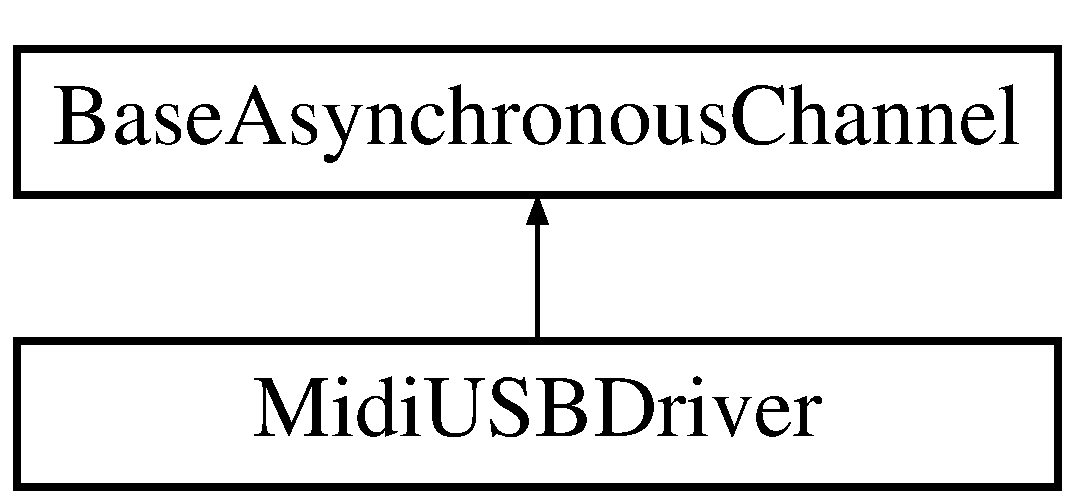
\includegraphics[height=2.000000cm]{structMidiUSBDriver}
\end{center}
\end{figure}
\subsection*{Public Attributes}
\begin{DoxyCompactItemize}
\item 
const struct \hyperlink{structMidiUSBDriverVMT}{Midi\+U\+S\+B\+Driver\+V\+MT} $\ast$ \hyperlink{structMidiUSBDriver_a284fcf42283692d4626add45fa497cd5}{vmt}\hypertarget{structMidiUSBDriver_a284fcf42283692d4626add45fa497cd5}{}\label{structMidiUSBDriver_a284fcf42283692d4626add45fa497cd5}

\begin{DoxyCompactList}\small\item\em Virtual Methods Table. \end{DoxyCompactList}\end{DoxyCompactItemize}


\subsection{Detailed Description}
Full duplex serial driver class. 

This class extends {\ttfamily Base\+Asynchronous\+Channel} by adding physical I/O queues. 

The documentation for this struct was generated from the following file\+:\begin{DoxyCompactItemize}
\item 
/c/\+Users/\+Pasquale/\+Documenti/\+Git\+Hub/axoloti/firmware/\hyperlink{midi__usb_8h}{midi\+\_\+usb.\+h}\end{DoxyCompactItemize}

\hypertarget{structMidiUSBDriverVMT}{}\section{Midi\+U\+S\+B\+Driver\+V\+MT Struct Reference}
\label{structMidiUSBDriverVMT}\index{Midi\+U\+S\+B\+Driver\+V\+MT@{Midi\+U\+S\+B\+Driver\+V\+MT}}


{\ttfamily Bulk\+U\+S\+B\+Driver} virtual methods table.  




{\ttfamily \#include $<$midi\+\_\+usb.\+h$>$}

Inheritance diagram for Midi\+U\+S\+B\+Driver\+V\+MT\+:\begin{figure}[H]
\begin{center}
\leavevmode
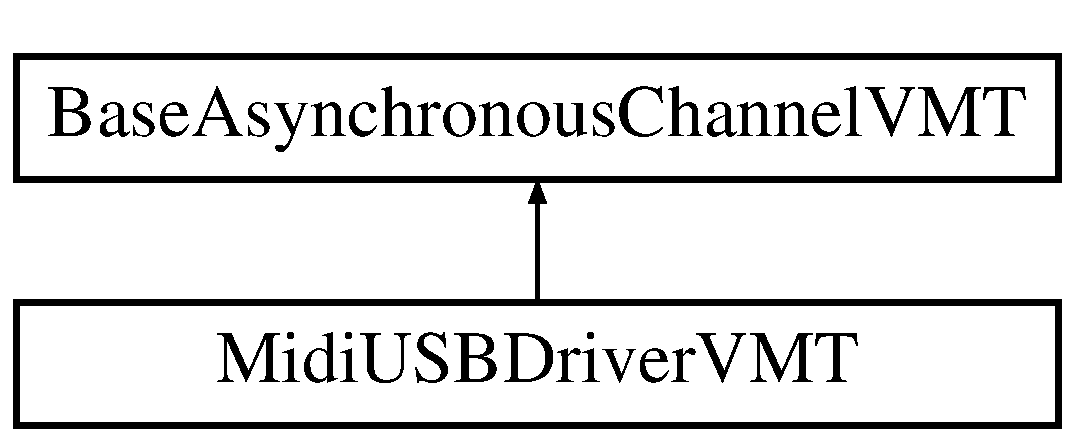
\includegraphics[height=2.000000cm]{structMidiUSBDriverVMT}
\end{center}
\end{figure}


\subsection{Detailed Description}
{\ttfamily Bulk\+U\+S\+B\+Driver} virtual methods table. 

The documentation for this struct was generated from the following file\+:\begin{DoxyCompactItemize}
\item 
/c/\+Users/pasquale.\+fersini/\+Documents/\+Git\+Hub/axoloti/firmware/\hyperlink{midi__usb_8h}{midi\+\_\+usb.\+h}\end{DoxyCompactItemize}

\hypertarget{structpatchMeta__t}{}\section{patch\+Meta\+\_\+t Struct Reference}
\label{structpatchMeta__t}\index{patch\+Meta\+\_\+t@{patch\+Meta\+\_\+t}}
\subsection*{Public Attributes}
\begin{DoxyCompactItemize}
\item 
fptr\+\_\+patch\+\_\+init\+\_\+t {\bfseries fptr\+\_\+patch\+\_\+init}
\item 
fptr\+\_\+patch\+\_\+dispose\+\_\+t {\bfseries fptr\+\_\+patch\+\_\+dispose}
\item 
fptr\+\_\+patch\+\_\+dsp\+\_\+process\+\_\+t {\bfseries fptr\+\_\+dsp\+\_\+process}
\item 
fptr\+\_\+patch\+\_\+midi\+\_\+in\+\_\+handler\+\_\+t {\bfseries fptr\+\_\+\+Midi\+In\+Handler}
\item 
fptr\+\_\+patch\+\_\+apply\+Preset\+\_\+t {\bfseries fptr\+\_\+apply\+Preset}
\item 
uint32\+\_\+t {\bfseries num\+P\+Ex}
\item 
Parameter\+Exchange\+\_\+t $\ast$ {\bfseries p\+P\+Exch}
\item 
int32\+\_\+t $\ast$ {\bfseries p\+Display\+Vector}
\item 
uint32\+\_\+t {\bfseries patch\+ID}
\item 
uint32\+\_\+t {\bfseries initpreset\+\_\+size}
\item 
void $\ast$ {\bfseries p\+Initpreset}
\item 
uint32\+\_\+t {\bfseries npresets}
\item 
uint32\+\_\+t {\bfseries npreset\+\_\+entries}
\item 
\hyperlink{structPresetParamChange__t}{Preset\+Param\+Change\+\_\+t} $\ast$ {\bfseries p\+Presets}
\end{DoxyCompactItemize}


The documentation for this struct was generated from the following file\+:\begin{DoxyCompactItemize}
\item 
/c/\+Users/pasquale.\+fersini/\+Documents/\+Git\+Hub/axoloti/firmware/\hyperlink{patch_8h}{patch.\+h}\end{DoxyCompactItemize}

\hypertarget{structPresetParamChange__t}{}\section{Preset\+Param\+Change\+\_\+t Struct Reference}
\label{structPresetParamChange__t}\index{Preset\+Param\+Change\+\_\+t@{Preset\+Param\+Change\+\_\+t}}
\subsection*{Public Attributes}
\begin{DoxyCompactItemize}
\item 
int32\+\_\+t {\bfseries pex\+Index}
\item 
int32\+\_\+t {\bfseries value}
\end{DoxyCompactItemize}


The documentation for this struct was generated from the following file\+:\begin{DoxyCompactItemize}
\item 
/c/\+Users/pasquale.\+fersini/\+Documents/\+Git\+Hub/axoloti/firmware/\hyperlink{patch_8h}{patch.\+h}\end{DoxyCompactItemize}

\chapter{File Documentation}
\hypertarget{codec_8h}{}\section{/c/\+Users/\+Pasquale/\+Documenti/\+Git\+Hub/axoloti/firmware/codec.h File Reference}
\label{codec_8h}\index{/c/\+Users/\+Pasquale/\+Documenti/\+Git\+Hub/axoloti/firmware/codec.\+h@{/c/\+Users/\+Pasquale/\+Documenti/\+Git\+Hub/axoloti/firmware/codec.\+h}}


Audio code high level interface functions.  


{\ttfamily \#include $<$stdint.\+h$>$}\\*
{\ttfamily \#include \char`\"{}axoloti\+\_\+defines.\+h\char`\"{}}\\*
\subsection*{Functions}
\begin{DoxyCompactItemize}
\item 
void \hyperlink{codec_8h_ab29f41fb27a45a93b99c9e278d2c23f5}{codec\+\_\+init} (void)\hypertarget{codec_8h_ab29f41fb27a45a93b99c9e278d2c23f5}{}\label{codec_8h_ab29f41fb27a45a93b99c9e278d2c23f5}

\begin{DoxyCompactList}\small\item\em Init audio codec. \end{DoxyCompactList}\item 
void \hyperlink{codec_8h_aa8e2755a23db1c5bf158d95e466e6021}{codec\+Stop} (void)\hypertarget{codec_8h_aa8e2755a23db1c5bf158d95e466e6021}{}\label{codec_8h_aa8e2755a23db1c5bf158d95e466e6021}

\begin{DoxyCompactList}\small\item\em Stop audio codec. \end{DoxyCompactList}\item 
void \hyperlink{codec_8h_a66abd2bd9fea55b99e4798e078cb3666}{computebufI} (int32\+\_\+t $\ast$inp, int32\+\_\+t $\ast$outp)
\begin{DoxyCompactList}\small\item\em Compute audio buffers. \end{DoxyCompactList}\item 
void \hyperlink{codec_8h_a11fe160b471a5e8f76614dfc7eeac808}{codec\+\_\+clearbuffer} (void)\hypertarget{codec_8h_a11fe160b471a5e8f76614dfc7eeac808}{}\label{codec_8h_a11fe160b471a5e8f76614dfc7eeac808}

\begin{DoxyCompactList}\small\item\em Clear audio codec buffer. \end{DoxyCompactList}\end{DoxyCompactItemize}
\subsection*{Variables}
\begin{DoxyCompactItemize}
\item 
int32\+\_\+t {\bfseries buf} \mbox{[}B\+U\+F\+S\+I\+ZE $\ast$2\mbox{]}\hypertarget{codec_8h_a3a8133ede80d26c722b224dfbf478d28}{}\label{codec_8h_a3a8133ede80d26c722b224dfbf478d28}

\item 
int32\+\_\+t {\bfseries buf2} \mbox{[}B\+U\+F\+S\+I\+ZE $\ast$2\mbox{]}\hypertarget{codec_8h_a7658fb8a235ed1348096a61b512a289e}{}\label{codec_8h_a7658fb8a235ed1348096a61b512a289e}

\item 
int32\+\_\+t {\bfseries rbuf} \mbox{[}B\+U\+F\+S\+I\+ZE $\ast$2\mbox{]}\hypertarget{codec_8h_a63c7dc43eda2f1c73eabc19a584f146b}{}\label{codec_8h_a63c7dc43eda2f1c73eabc19a584f146b}

\item 
int32\+\_\+t {\bfseries rbuf2} \mbox{[}B\+U\+F\+S\+I\+ZE $\ast$2\mbox{]}\hypertarget{codec_8h_a538366b85246e4b4465d92250e6acbe7}{}\label{codec_8h_a538366b85246e4b4465d92250e6acbe7}

\end{DoxyCompactItemize}


\subsection{Detailed Description}
Audio code high level interface functions. 



\subsection{Function Documentation}
\index{codec.\+h@{codec.\+h}!computebufI@{computebufI}}
\index{computebufI@{computebufI}!codec.\+h@{codec.\+h}}
\subsubsection[{\texorpdfstring{computebuf\+I(int32\+\_\+t $\ast$inp, int32\+\_\+t $\ast$outp)}{computebufI(int32_t *inp, int32_t *outp)}}]{\setlength{\rightskip}{0pt plus 5cm}void computebufI (
\begin{DoxyParamCaption}
\item[{int32\+\_\+t $\ast$}]{inp, }
\item[{int32\+\_\+t $\ast$}]{outp}
\end{DoxyParamCaption}
)}\hypertarget{codec_8h_a66abd2bd9fea55b99e4798e078cb3666}{}\label{codec_8h_a66abd2bd9fea55b99e4798e078cb3666}


Compute audio buffers. 


\begin{DoxyParams}[1]{Parameters}
\mbox{\tt in}  & {\em $\ast$inp} & Pointer to input buffer. \\
\hline
\mbox{\tt out}  & {\em $\ast$outp} & Pointer to output buffer. \\
\hline
\end{DoxyParams}

\hypertarget{midi__usb_8h}{}\section{/c/\+Users/pasquale.fersini/\+Documents/\+Git\+Hub/axoloti/firmware/midi\+\_\+usb.h File Reference}
\label{midi__usb_8h}\index{/c/\+Users/pasquale.\+fersini/\+Documents/\+Git\+Hub/axoloti/firmware/midi\+\_\+usb.\+h@{/c/\+Users/pasquale.\+fersini/\+Documents/\+Git\+Hub/axoloti/firmware/midi\+\_\+usb.\+h}}


M\+I\+DI U\+SB Driver macros and structures.  


{\ttfamily \#include \char`\"{}midi.\+h\char`\"{}}\\*
\subsection*{Classes}
\begin{DoxyCompactItemize}
\item 
struct \hyperlink{structMidiUSBConfig}{Midi\+U\+S\+B\+Config}
\begin{DoxyCompactList}\small\item\em Bulk U\+SB Driver configuration structure. \end{DoxyCompactList}\item 
struct \hyperlink{structMidiUSBDriverVMT}{Midi\+U\+S\+B\+Driver\+V\+MT}
\begin{DoxyCompactList}\small\item\em {\ttfamily Bulk\+U\+S\+B\+Driver} virtual methods table. \end{DoxyCompactList}\item 
struct \hyperlink{structMidiUSBDriver}{Midi\+U\+S\+B\+Driver}
\begin{DoxyCompactList}\small\item\em Full duplex serial driver class. \end{DoxyCompactList}\end{DoxyCompactItemize}
\subsection*{Macros}
\begin{DoxyCompactItemize}
\item 
\#define \hyperlink{group__MIDI__USB_ga8cfb956039dff17bc67f80137c28bcbb}{\+\_\+midi\+\_\+usb\+\_\+driver\+\_\+data}
\begin{DoxyCompactList}\small\item\em {\ttfamily \hyperlink{structMidiUSBDriver}{Midi\+U\+S\+B\+Driver}} specific data. \end{DoxyCompactList}\item 
\#define \hyperlink{group__MIDI__USB_gaed42fc468f948c258e107f51e5f89a07}{\+\_\+midi\+\_\+usb\+\_\+driver\+\_\+methods}~\+\_\+base\+\_\+asynchronous\+\_\+channel\+\_\+methods
\begin{DoxyCompactList}\small\item\em {\ttfamily Bulk\+U\+S\+B\+Driver} specific methods. \end{DoxyCompactList}\end{DoxyCompactItemize}
\begin{Indent}{\bf M\+I\+D\+I\+\_\+\+U\+SB configuration options}\par
\begin{DoxyCompactItemize}
\item 
\#define \hyperlink{group__MIDI__USB_ga76b9bd9d7068efe165b409fad9c63fc5}{M\+I\+D\+I\+\_\+\+U\+S\+B\+\_\+\+B\+U\+F\+F\+E\+R\+S\+\_\+\+S\+I\+ZE}~64
\begin{DoxyCompactList}\small\item\em Midi U\+SB buffers size. \end{DoxyCompactList}\end{DoxyCompactItemize}
\end{Indent}
\subsection*{Typedefs}
\begin{DoxyCompactItemize}
\item 
typedef struct \hyperlink{structMidiUSBDriver}{Midi\+U\+S\+B\+Driver} \hyperlink{group__MIDI__USB_ga6f6e4a9a3715905f731618419195caeb}{Midi\+U\+S\+B\+Driver}
\begin{DoxyCompactList}\small\item\em Structure representing a bulk U\+SB driver. \end{DoxyCompactList}\end{DoxyCompactItemize}
\subsection*{Enumerations}
\begin{DoxyCompactItemize}
\item 
enum \hyperlink{group__MIDI__USB_gaf100a937cc2fe8a2a694884d6ec92485}{mdustate\+\_\+t} \{ \hyperlink{group__MIDI__USB_ggaf100a937cc2fe8a2a694884d6ec92485a872997df0e7465da70e4f1e37b3507ec}{M\+D\+U\+\_\+\+U\+N\+I\+N\+IT} = 0, 
\hyperlink{group__MIDI__USB_ggaf100a937cc2fe8a2a694884d6ec92485accf69965e5109667e5593415ca70fe06}{M\+D\+U\+\_\+\+S\+T\+OP} = 1, 
\hyperlink{group__MIDI__USB_ggaf100a937cc2fe8a2a694884d6ec92485a87df2c76063f4f72e57ec1a82d21a618}{M\+D\+U\+\_\+\+R\+E\+A\+DY} = 2
 \}\begin{DoxyCompactList}\small\item\em Driver state machine possible states. \end{DoxyCompactList}
\end{DoxyCompactItemize}
\subsection*{Functions}
\begin{DoxyCompactItemize}
\item 
void {\bfseries mdu\+Init} (void)
\item 
void {\bfseries mdu\+Object\+Init} (\hyperlink{structMidiUSBDriver}{Midi\+U\+S\+B\+Driver} $\ast$sdp)
\item 
void {\bfseries mdu\+Start} (\hyperlink{structMidiUSBDriver}{Midi\+U\+S\+B\+Driver} $\ast$mdup, const \hyperlink{structMidiUSBConfig}{Midi\+U\+S\+B\+Config} $\ast$config)
\item 
void {\bfseries mdu\+Stop} (\hyperlink{structMidiUSBDriver}{Midi\+U\+S\+B\+Driver} $\ast$mdup)
\item 
void {\bfseries mdu\+Configure\+HookI} (\hyperlink{structMidiUSBDriver}{Midi\+U\+S\+B\+Driver} $\ast$bdup)
\item 
bool\+\_\+t {\bfseries mdu\+Requests\+Hook} (U\+S\+B\+Driver $\ast$usbp)
\item 
void {\bfseries mdu\+Data\+Transmitted} (U\+S\+B\+Driver $\ast$usbp, usbep\+\_\+t ep)
\item 
void {\bfseries mdu\+Data\+Received} (U\+S\+B\+Driver $\ast$usbp, usbep\+\_\+t ep)
\item 
void {\bfseries midi\+\_\+usb\+\_\+\+Midi\+Send1} (uint8\+\_\+t port, uint8\+\_\+t b0)
\item 
void {\bfseries midi\+\_\+usb\+\_\+\+Midi\+Send2} (uint8\+\_\+t port, uint8\+\_\+t b0, uint8\+\_\+t b1)
\item 
void {\bfseries midi\+\_\+usb\+\_\+\+Midi\+Send3} (uint8\+\_\+t port, uint8\+\_\+t b0, uint8\+\_\+t b1, uint8\+\_\+t b2)
\end{DoxyCompactItemize}


\subsection{Detailed Description}
M\+I\+DI U\+SB Driver macros and structures. 


\hypertarget{patch_8h}{}\section{/c/\+Users/\+Pasquale/\+Documenti/\+Git\+Hub/axoloti/firmware/patch.h File Reference}
\label{patch_8h}\index{/c/\+Users/\+Pasquale/\+Documenti/\+Git\+Hub/axoloti/firmware/patch.\+h@{/c/\+Users/\+Pasquale/\+Documenti/\+Git\+Hub/axoloti/firmware/patch.\+h}}


Axoloti Core D\+SP patch macros and structures.  


{\ttfamily \#include $<$stdint.\+h$>$}\\*
{\ttfamily \#include \char`\"{}ch.\+h\char`\"{}}\\*
{\ttfamily \#include \char`\"{}hal.\+h\char`\"{}}\\*
{\ttfamily \#include \char`\"{}ui.\+h\char`\"{}}\\*
{\ttfamily \#include \char`\"{}axoloti\+\_\+board.\+h\char`\"{}}\\*
{\ttfamily \#include \char`\"{}ff.\+h\char`\"{}}\\*
{\ttfamily \#include \char`\"{}midi.\+h\char`\"{}}\\*
{\ttfamily \#include \char`\"{}crc32.\+h\char`\"{}}\\*
{\ttfamily \#include \char`\"{}exceptions.\+h\char`\"{}}\\*
\subsection*{Classes}
\begin{DoxyCompactItemize}
\item 
struct \hyperlink{structPresetParamChange__t}{Preset\+Param\+Change\+\_\+t}
\item 
struct \hyperlink{structpatchMeta__t}{patch\+Meta\+\_\+t}
\end{DoxyCompactItemize}
\subsection*{Macros}
\begin{DoxyCompactItemize}
\item 
\#define {\bfseries P\+A\+T\+C\+H\+M\+A\+I\+N\+L\+OC}~0x20011000
\item 
\#define {\bfseries P\+A\+T\+C\+H\+F\+L\+A\+S\+H\+L\+OC}~0x080\+E0000
\item 
\#define {\bfseries P\+A\+T\+C\+H\+F\+L\+A\+S\+H\+S\+I\+ZE}~0x\+B000
\end{DoxyCompactItemize}
\subsection*{Typedefs}
\begin{DoxyCompactItemize}
\item 
typedef void($\ast$ {\bfseries fptr\+\_\+patch\+\_\+init\+\_\+t}) (int32\+\_\+t fw\+ID)
\item 
typedef void($\ast$ {\bfseries fptr\+\_\+patch\+\_\+dispose\+\_\+t}) (void)
\item 
typedef void($\ast$ {\bfseries fptr\+\_\+patch\+\_\+dsp\+\_\+process\+\_\+t}) (int32\+\_\+t $\ast$, int32\+\_\+t $\ast$)
\item 
typedef void($\ast$ {\bfseries fptr\+\_\+patch\+\_\+midi\+\_\+in\+\_\+handler\+\_\+t}) (midi\+\_\+device\+\_\+t dev, uint8\+\_\+t port, uint8\+\_\+t, uint8\+\_\+t, uint8\+\_\+t)
\item 
typedef void($\ast$ {\bfseries fptr\+\_\+patch\+\_\+apply\+Preset\+\_\+t}) (int32\+\_\+t)
\end{DoxyCompactItemize}
\subsection*{Enumerations}
\begin{DoxyCompactItemize}
\item 
enum \hyperlink{group__PATCH_ga3bcfa0e2fd6136eb75131fe31d3c0ecf}{load\+Patch\+Index\+\_\+t} \{ \\*
\hyperlink{group__PATCH_gga3bcfa0e2fd6136eb75131fe31d3c0ecfa4ea978b80c692bb277f7219bc4941cac}{S\+T\+A\+R\+T\+\_\+\+SD} = -\/1, 
\hyperlink{group__PATCH_gga3bcfa0e2fd6136eb75131fe31d3c0ecfa14501ea9e7b84bf1917c39939a4fe295}{S\+T\+A\+R\+T\+\_\+\+F\+L\+A\+SH} = -\/2, 
\hyperlink{group__PATCH_gga3bcfa0e2fd6136eb75131fe31d3c0ecfabf80358ff9809b38be4b95d6d157914d}{B\+Y\+\_\+\+F\+I\+L\+E\+N\+A\+ME} = -\/3, 
\hyperlink{group__PATCH_gga3bcfa0e2fd6136eb75131fe31d3c0ecfa5810f7a85a06138a19e6f548273a6927}{L\+I\+VE} = -\/4, 
\\*
\hyperlink{group__PATCH_gga3bcfa0e2fd6136eb75131fe31d3c0ecfaf096820742c38363e9d6c33e7c932780}{U\+N\+I\+N\+I\+T\+I\+A\+L\+I\+Z\+ED} = -\/5
 \}\begin{DoxyCompactList}\small\item\em Patch source. \end{DoxyCompactList}
\item 
enum {\bfseries patch\+Status\+\_\+t} \{ {\bfseries R\+U\+N\+N\+I\+NG} = 0, 
{\bfseries S\+T\+O\+P\+P\+ED} = 1, 
{\bfseries S\+T\+O\+P\+P\+I\+NG} = 2, 
{\bfseries S\+T\+A\+R\+T\+F\+A\+I\+L\+ED} = 3
 \}\hypertarget{group__PATCH_ga4fae02d17665f4d292b175458d7a8ea0}{}\label{group__PATCH_ga4fae02d17665f4d292b175458d7a8ea0}

\end{DoxyCompactItemize}
\subsection*{Functions}
\begin{DoxyCompactItemize}
\item 
void {\bfseries Init\+Patch0} (void)
\item 
int {\bfseries Start\+Patch} (void)
\item 
void {\bfseries Stop\+Patch} (void)
\item 
void {\bfseries start\+\_\+dsp\+\_\+thread} (void)
\item 
void {\bfseries Start\+Load\+Patch\+Tread} (void)
\item 
void {\bfseries Load\+Patch} (const char $\ast$name)
\item 
void {\bfseries Load\+Patch\+Start\+SD} (void)
\item 
void {\bfseries Load\+Patch\+Start\+Flash} (void)
\item 
void {\bfseries Load\+Patch\+Indexed} (uint32\+\_\+t index)
\item 
\hyperlink{group__PATCH_ga3bcfa0e2fd6136eb75131fe31d3c0ecf}{load\+Patch\+Index\+\_\+t} {\bfseries Get\+Index\+Of\+Current\+Patch} (void)
\item 
int {\bfseries get\+\_\+\+U\+S\+B\+H\+\_\+\+L\+L\+\_\+\+Get\+U\+R\+B\+State} (void)
\item 
int {\bfseries get\+\_\+\+U\+S\+B\+H\+\_\+\+L\+L\+\_\+\+Submit\+U\+RB} (void)
\end{DoxyCompactItemize}
\subsection*{Variables}
\begin{DoxyCompactItemize}
\item 
\hyperlink{structpatchMeta__t}{patch\+Meta\+\_\+t} {\bfseries patch\+Meta}
\item 
int {\bfseries dsp\+Load\+Pct}
\item 
\hyperlink{group__PATCH_ga3bcfa0e2fd6136eb75131fe31d3c0ecf}{load\+Patch\+Index\+\_\+t} {\bfseries load\+Patch\+Index}
\item 
volatile patch\+Status\+\_\+t {\bfseries patch\+Status}
\item 
int8\+\_\+t {\bfseries hid\+\_\+buttons} \mbox{[}8\mbox{]}
\item 
int8\+\_\+t {\bfseries hid\+\_\+mouse\+\_\+x}
\item 
int8\+\_\+t {\bfseries hid\+\_\+mouse\+\_\+y}
\end{DoxyCompactItemize}


\subsection{Detailed Description}
Axoloti Core D\+SP patch macros and structures. 

Copyright (C) 2013, 2014 Johannes Taelman

This file is part of Axoloti.

Axoloti is free software\+: you can redistribute it and/or modify it under the terms of the G\+NU General Public License as published by the Free Software Foundation, either version 3 of the License, or (at your option) any later version.

Axoloti is distributed in the hope that it will be useful, but W\+I\+T\+H\+O\+UT A\+NY W\+A\+R\+R\+A\+N\+TY; without even the implied warranty of M\+E\+R\+C\+H\+A\+N\+T\+A\+B\+I\+L\+I\+TY or F\+I\+T\+N\+E\+SS F\+OR A P\+A\+R\+T\+I\+C\+U\+L\+AR P\+U\+R\+P\+O\+SE. See the G\+NU General Public License for more details.

You should have received a copy of the G\+NU General Public License along with Axoloti. If not, see \href{http://www.gnu.org/licenses/}{\tt http\+://www.\+gnu.\+org/licenses/}. 
%--- End generated contents ---

% Index
\backmatter
\newpage
\phantomsection
\clearemptydoublepage
\addcontentsline{toc}{chapter}{Index}
\printindex

\end{document}
